\documentclass[12pt]{article}
\usepackage[english]{babel}
\usepackage{color,soul}
\usepackage{apacite} 
\bibliographystyle{apacite}
\usepackage{url}
\usepackage[titletoc]{appendix}
\usepackage[utf8x]{inputenc}
\usepackage{lmodern}
\usepackage{listings}
\usepackage{amsmath}
\usepackage{courier}
\usepackage{wrapfig}
\usepackage[export]{adjustbox}
\usepackage[bottom]{footmisc}
\usepackage{graphicx}
\usepackage{hyperref}
\usepackage{pdfpages}
\usepackage{comment}
\graphicspath{{images/}}
\usepackage{parskip}
\usepackage{flafter}
\usepackage{colortbl}
\usepackage{fancyhdr}
\usepackage{csvsimple}
\usepackage{booktabs}
\usepackage{longtable}
\usepackage{multirow}
\usepackage{vmargin}
\usepackage{listings}
\usepackage{pgfplotstable,filecontents}
\usepackage{natbib}
\usepackage{subfigure}
\usepackage{graphicx}
\usepackage{sidecap}
\usepackage{floatrow}
\usepackage{framed}
\usepackage[T1]{fontenc}
\usepackage{babel}
\usepackage{listings}
\usepackage[font=small,labelfont=bf]{caption}
\newfloatcommand{capbtabbox}{table}[][\FBwidth]
\usepackage{blindtext}
\usepackage[section]{placeins}
\usepackage{csvsimple}
\setlength{\bibsep}{5.0pt}
\pgfplotsset{compat=1.9}% supress warning
\setmarginsrb{2.5cm}{1.5cm}{2.5 cm}{1.5 cm}{1.5 cm}{1 cm}{1 cm}{1.5 cm}
\usepackage{color}
\usepackage{minted}
\usepackage{array}
\newcolumntype{L}[1]{>{\raggedright\let\newline\\\arraybackslash\hspace{0pt}}m{#1}}
\newcolumntype{C}[1]{>{\centering\let\newline\\\arraybackslash\hspace{0pt}}m{#1}}
\newcolumntype{R}[1]{>{\raggedleft\let\newline\\\arraybackslash\hspace{0pt}}m{#1}}
\definecolor{dkgreen}{rgb}{0,0.6,0}
\definecolor{gray}{rgb}{0.5,0.5,0.5}
\definecolor{mauve}{rgb}{0.58,0,0.82}
\definecolor{black}{rgb}{0,0,0}
\definecolor{white}{rgb}{1,1,1}
\definecolor{blue}{rgb}{0,0,1}
\definecolor{red}{rgb}{1,0,0}
\lstset{ 
  language=C++,                         
  basicstyle=\scriptsize,       
  numbers=left,                   		% where to put the line-numbers
  numberstyle=\tiny\color{gray},  	% the style that is used for the line-numbers
  stepnumber=1,                   		% the step between two line-numbers. If it's 1, each line will be numbered
  numbersep=5pt,                  		% how far the line-numbers are from the code
  backgroundcolor=\color{white},  	% choose the background color. must add \usepackage{color}
  showspaces=false,               		% show spaces adding particular underscores
  showstringspaces=false,        		 % underline spaces within strings
  showtabs=false,                		 % show tabs within strings adding particular underscores
  frame=single,                  			 % adds a frame around the code
  rulecolor=\color{black},       		 % if not set, the frame-color may be changed on line-breaks within not-black text (e.g. commens (green here))
  tabsize=2,                      			% sets default tabsize to 2 spaces
  captionpos=b,                   		% sets the caption-position to bottom
  breaklines=true,               		 % sets automatic line breaking
  breakatwhitespace=false,       		 % sets if automatic breaks should only happen at whitespace
  title=\lstname,                 			% show the filename of files included with \lstinputlisting;
                                 				 % also try caption instead of title
  keywordstyle=\color{blue},      		% keyword style
  commentstyle=\color{dkgreen},  	 % comment style
  stringstyle=\color{mauve},      		% string literal style
  escapeinside={\%*}{*)},         		% if you want to add a comment within your code
  morekeywords={*,...}           		 % if you want to add more keywords to the set
} 

\newtheorem{esti}{Theorem}[section]
\title{CS3201/2 Iteration 2}					% Title
% * <akankshita.dash@u.nus.edu> 2017-09-06T05:26:27.242Z:
%
% ^.	

\makeatletter
\let\thetitle\@title
\let\theauthor\@author
\let\thedate\@date
\makeatother
\author{}
\pagestyle{fancy}
\fancyhf{}
\rhead{\theauthor}
\lhead{\thetitle}
\cfoot{\thepage}
\usepackage{setspace}
\begin{document}
\doublespacing
%%%%%%%%%%%%%%%%%%%%%%%%%%%%%%%%%%%%%%%%%%%%%%%%%%%%%%%%%%%%%%%%%%%%%%%%%%%%%%%%%%%%%%%%%

%%%%%%%%%%%%%%%%%%%%%%%%%%%%%%%%%%%%%%%%%%%%%%%%%%%%%%%%%%%%%%%%%%%%%%%%%%%%%%%%%%%%%%%%%

\begin{titlepage}
	\centering
    
\includegraphics[width = 0.4\textwidth]{logo1.jpg}\\[0.4cm]	% University Logo
    \textsc{ National University of Singapore}\\[0.2 cm]	% University Name
	\rule{\linewidth}{0.2 mm} \\[0.1 cm]
	{ \huge \bfseries \thetitle}\\
    \rule{\linewidth}{0.2 mm} \\[0.2 cm]
			\begin{center} 
            \textbf{16th October 2017}\\[0.7cm]
			\textbf { SEM 1, AY2017/2018}\\[0.7cm]
			\emph{Submitted By :} \\[0.1cm]
           
      \textbf{\underline{Team 11}}    
      \subsubsection*{Consultation Hour: Tuesday, 1:00-2:00 pm}
 \begin{table}[htbp]
\begin{tabular}{|c|c|c|}
\hline
\textbf{Team Member} & \textbf{E-mail} & \textbf{Phone number}\\\hline
Akankshita Dash & akankshita.dash@u.nus.edu & 84010419  \\
\hline
Chua Ping Chan & a0126623@u.nus.edu & 90876406 \\
\hline
Lau Wen Hao & a0121528@u.nus.edu & 84991295  \\
\hline
Marcus Ng & marcusngwenjian@u.nus.edu
 & 97502493  \\
\hline
Zhang Ying & e0006954@u.nus.edu
 & 82289895  \\
\hline
Zhuang Lei & e0003940@u.nus.edu
 & 98374236 \\
\hline
\end{tabular}
\end{table}
		    \end{center}
        


\end{titlepage}

%%%%%%%%%%%%%%%%%%%%%%%%%%%%%%%%%%%%%%%%%%%%%%%%%%%%%%%%%%%%%%%%%%%%%%%%%%%%%%%%%%%%%%%%%

%%%%%%%%%%%%%%%%%%%%%%%%%%%%%%%%%%%%%%%%%%%%%%%%%%%%%%%%%%%%%%%%%%%%%%%%%%%%%%%%%%%%%%%%%
\tableofcontents
\vspace{200mm}
\section{Scope of SPA Implementation}
Our prototype for SPA meets all the requirements for Iteration 2 and is a fully operational mini-SPA.
\subsection{Parser}
Our \textbf{SPA tool} is now able to parse if-else statements, call statements and procedures in addition to previous parsing of multiple statements, assignments and while loops. 
\subsection{PKB}
PKB now supports \textbf{Calls,Calls*, Next, Next*, Pattern If, Pattern While} as well as \textbf{Modifies} and \textbf{Uses} for procedures, in addition to previous implementations of \textbf{Follows, Follows*, Parent, Parent*, Uses, Modifies and Pattern}
\subsection{PQL}
The QueryProcessor is able to evaluate PQL Queries with multiple \textbf{such that, pattern, and} and \textbf{with} clauses. It can also handle selection of \textbf{BOOLEAN} types.
\section{Development Plan}
\subsection{Development Plan for SPA}
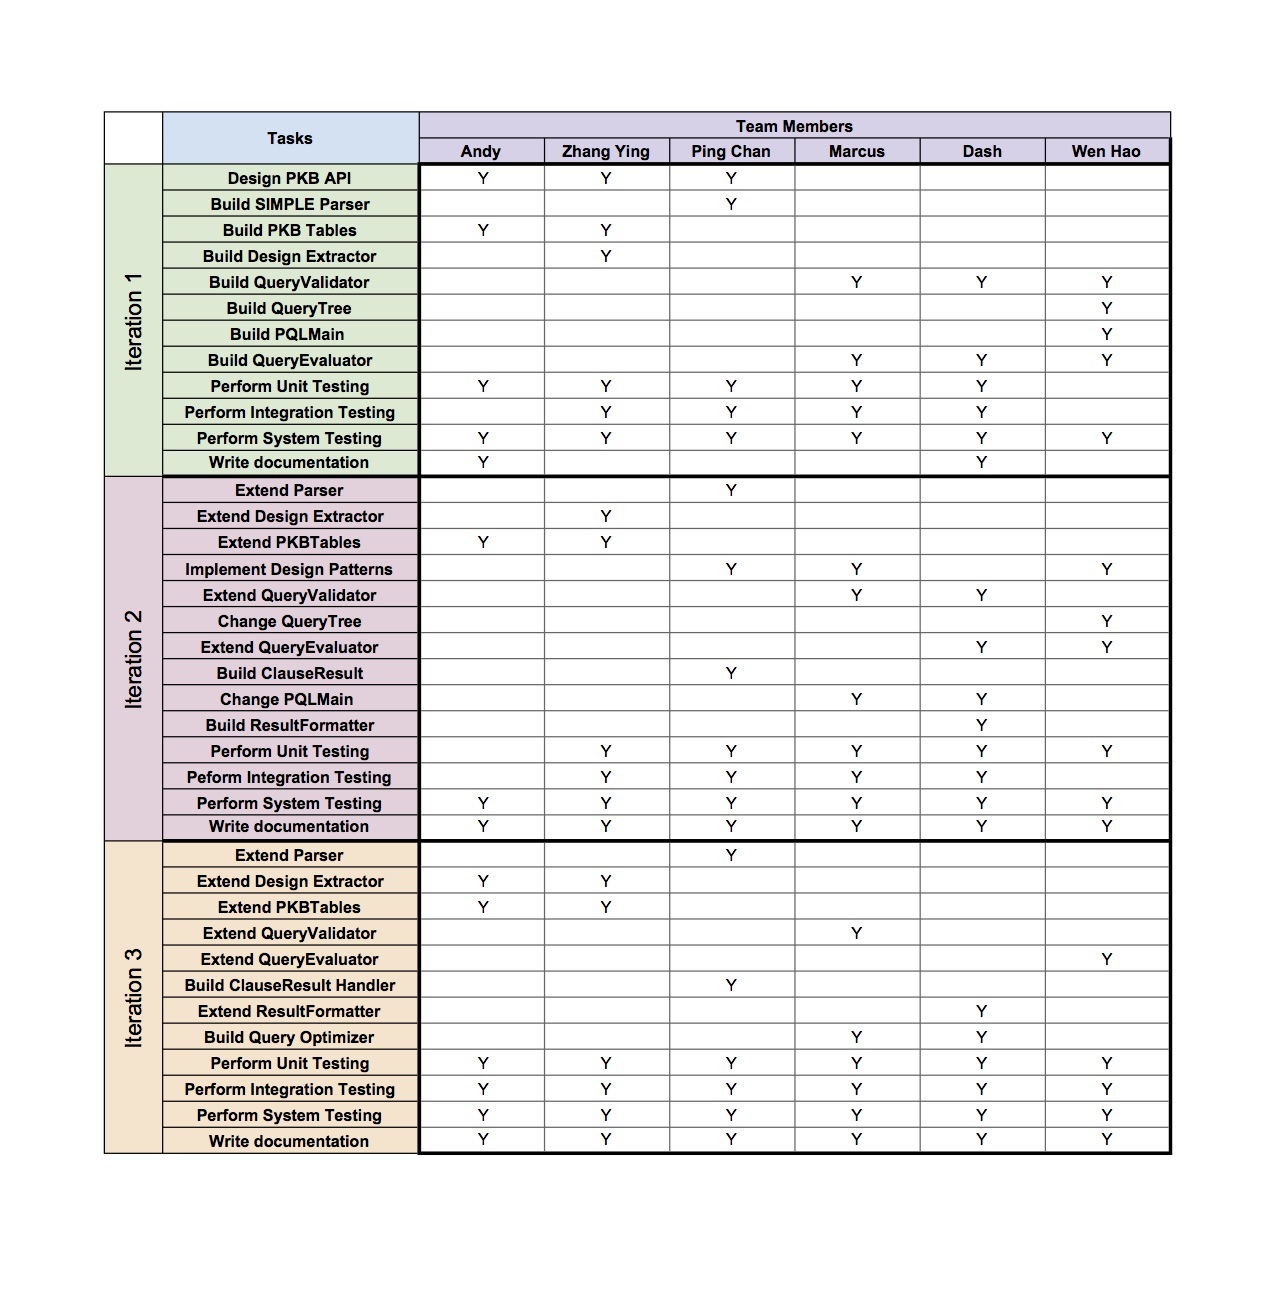
\includegraphics[width = 1.4\textwidth,center]{DevPlan.jpg}
\subsection{Development Plan for Iteration 2}
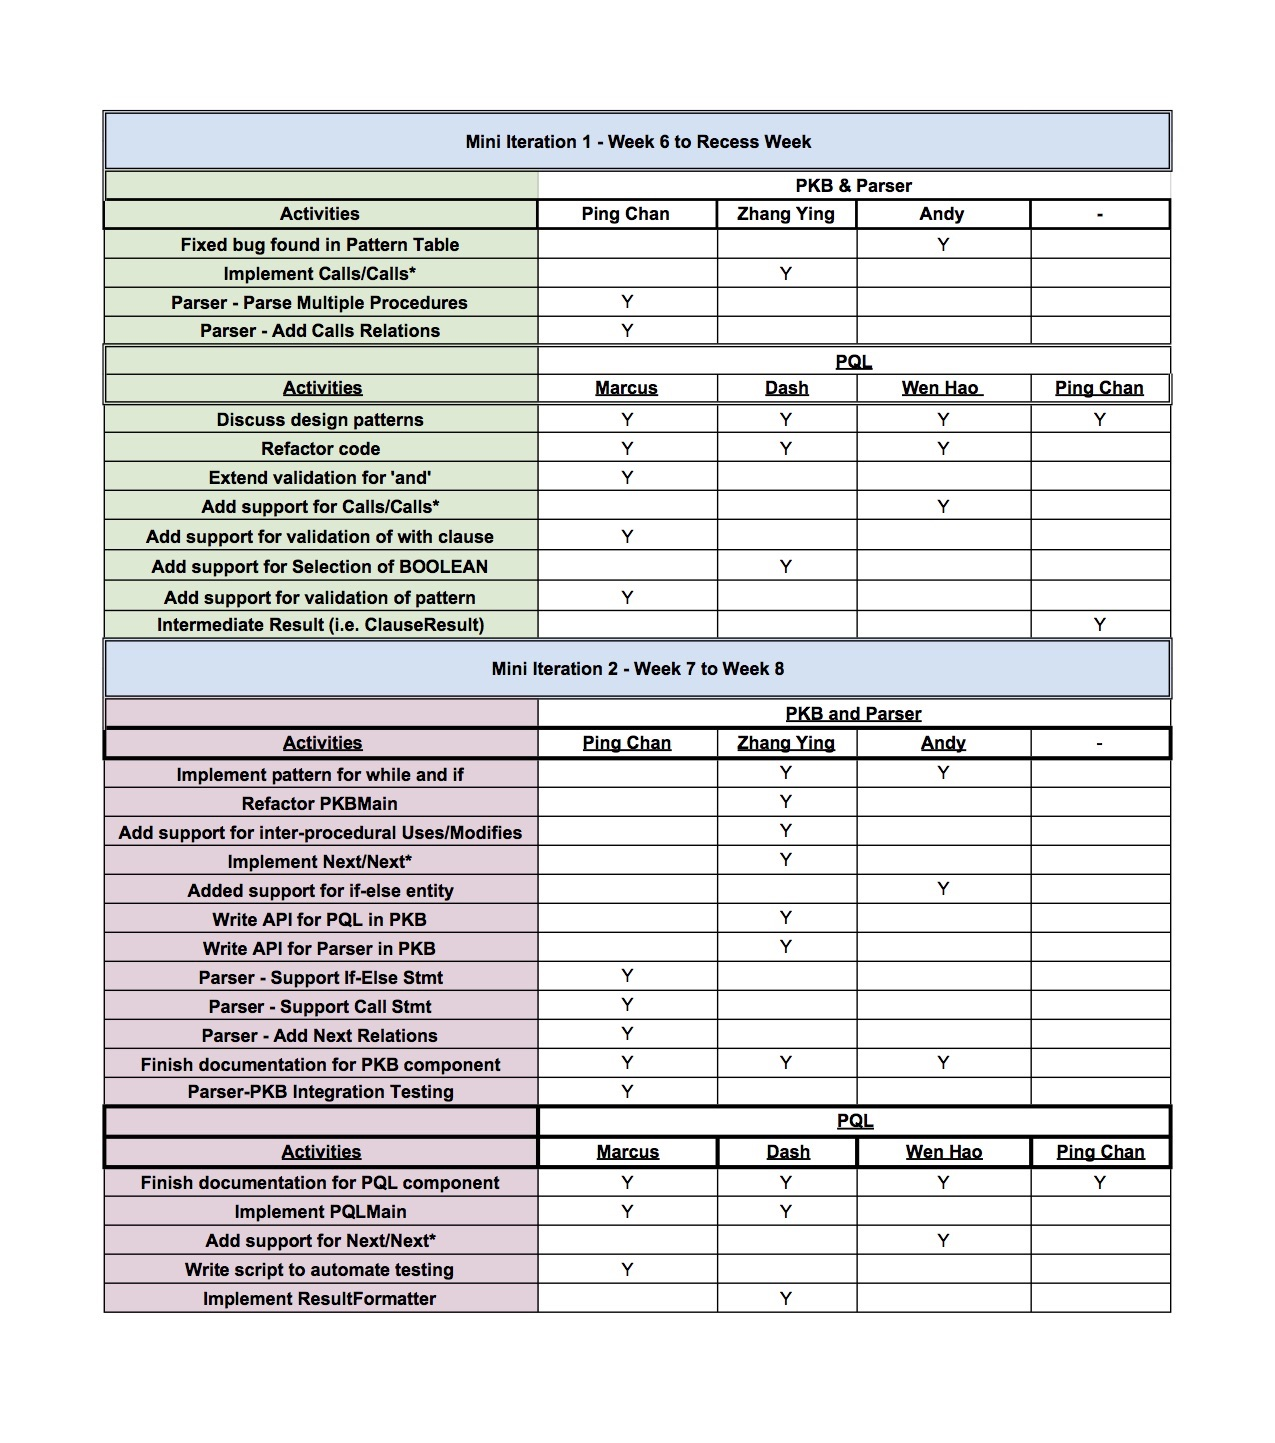
\includegraphics[width = 1.2\textwidth,center]{Iteration2.jpg}
\section{SPA Design}
\subsection{Overview}
\begin{figure}[!htb].
\centering
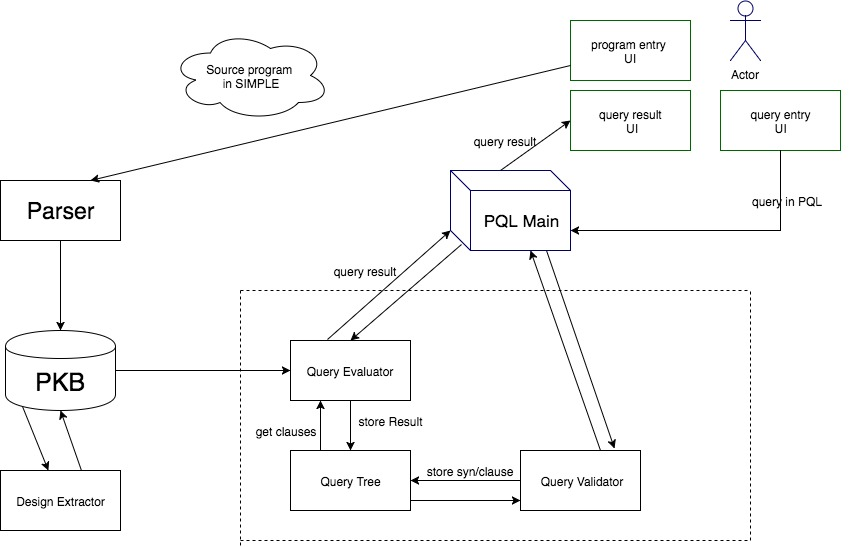
\includegraphics[width=0.8\textwidth]{Architecture_Diagram.jpg}
\caption{\label{fig:Architecture}Main components of SPA}
\end{figure}
In  SPA, there are two main components:
\begin{enumerate}
\item Program Knowledge Base (PKB)
\item Program Query Language (PQL)
\end{enumerate}

Our SPA design is very similar to the original proposed design. In addition, to the proposed components, we have implemented a PQL Main, which controls the flow of all the other components in PQL and decides the sequence during query processing.

For iteration 3, we will implement Query Optimizer, which will come re-order clauses in order to optimize evaluation. It will work after Query Validator and before Query Evaluator.

\subsection{Design of SPA Components}

\subsubsection{Parser }
In SPA, Parser is responsible for parsing a given SIMPLE source code, validating the syntax, extracting information and storing it in PKB.

Whenever the Parser detects a syntax error, it will stop parsing the SIMPLE source and display an error feedback message to the user. It is only if the SIMPLE source code is syntactically correct, that the Parser will finish parsing and allow queries to be evaluated.

At the beginning of the parsing process, the Parser reads a given SIMPLE source file into a concatenated string, which is stored in-memory in a class attribute.

After the SIMPLE source content is extracted into a concatenated string, the Parser will make one parse just to ensure all the braces pairs up correctly. If there is a mismatch in the way the braces pair-up, the Parser will output a feedback message to indicate the syntax error and stop parsing at once.

If all the braces are paired up well, the Parser is now ready to Parse the SIMPLE source contents line by line. The Parser implemented is a predictive recursive descent parser, whereby the concatenated SOURCE string will be tokenized; the Parser starts by reading a token, and then determines what is the next token to expect.
\begin{center}
\fbox{\begin{minipage}{40em}
\begin{center}Parser’s Tokenizer\end{center}
The tokenizer of the parser is made such that if given a SIMPLE program: \linebreak
\texttt{procedure First \{
   \newline abc123 = 100 * x3;
\newline\} }
\newline The tokenizer will break the string down to a list of tokens containing:
‘procedure’, ‘First’, ‘\{’, ‘abc123’, ‘=’, ‘$100$’, ‘*’, ‘$x3$’, ‘;’ and ‘\}’.
Any interleaving whitespace will be ignored.
\end{minipage}}
\end{center}
\vspace{10mm}For example, at the very beginning of the SIMPLE source, the Parser invokes a member function that parses procedure, and expects the upcoming token to be the keyword “procedure”. If the first token indeed matches the keyword, the Parser will move on to the next token and validate whether it is a valid procedure name or not, according to the SIMPLE grammar rules. If it is valid, the Parser will add the name of procedure into PKB. It will then expect an open brace character ‘\{‘ next, and so on.

Similar to parsing procedure, the Parser contains various methods to parse different entities such as statement lists, assignment statements, call statements, while statements and if-else statements. Each of these methods will ensure the SIMPLE source satisfies the grammar rules, e.g. correct operands, correct expressions in assignment statements, etc. If any syntax error is detected, Parser will throw an exception and stop parsing.

After the Parser finishes parsing a SIMPLE source, it signals to PKB that it's finished, so that the Design Extractor within PKB starts computing transitive relations, e.g. Follows*, Parent*, Calls*, Next* and inter-procedural relations such as Uses and Modifies.

\textbf{Uses/Modifies Relation:} The Parser adds the Modifies and Uses relationship into PKB as and when the Parser parsers the relevant statements. No additional data structures are required to store any information for adding Uses/Modifies relations.

\textbf{Follows Relation:} The Parser maintains a stack of statements in order to add Follows relations to PKB. Each inner stacks represents the statement list within a code block in the correct order, and the outer stack is used to store the information of nested statement lists due to container statements.

As each inner stack represents a statement list with statements in the correct order, at the end of a code block, Parser can pop the top-most statement list in the stack and process it by setting the Follows relation based on the sequence of statements in the code block.
\newpage
Consider the following source code:
\begin{center}
\fbox{\begin{minipage}{35em}
\texttt{procedure First \{
\newline1 \hspace{3mm}	i = 1;
\newline2 \hspace{3mm}	b = 200;
\newline3 \hspace{3mm} c = a;
\newline4 \hspace{3mm} while a \{
\newline5 \hspace{12mm}		c = b - 5;
\newline6	\hspace{12mm}	b = c - a;
\newline7	\hspace{12mm}	x = x + 1; 
\newline \phantom{he} \}
\newline    8 \hspace{3mm}  d = 300;
\}}
\end{minipage}}
\end{center}
\vspace{10mm}
The stack of statements stacks will be empty at first. While beginning to parse statement 1, since it is the first statement in a new statement list, an empty stack of statement will be created and pushed onto the stack of statements stacks. Statement 1, 2, 3 and 4 will then be pushed onto the inner stack in order. When parsing statement 5, as it is a new statement in a new nested statement list, another inner stack will be created. Statements 5, 6, 7 will then be added to this new inner stack and pushed into \_stackOfFollowsStack. At the end of parsing statement 7, upon exiting the code block of the while statement, the top stack (marked in green) will be popped, and the follows relation among statements 5, 6 and 7 will be added to PKB. Then, statement 8 will be pushed to the blue statements stack. At the end of parsing statement 8, the end of procedure is reached, therefore the blue stack will be popped and the Follows relations amongst statements 1, 2, 3, 4 and 8 will be added to the PKB.
\begin{figure}[htbp]
  \caption{Keeping Track of Follows Relationship}
  \centering
    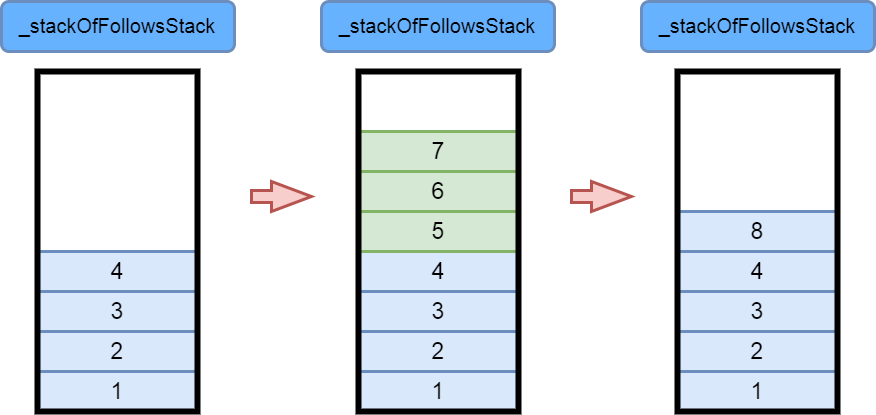
\includegraphics[width=0.7\textwidth]{Parser_AddingFollowsRelationToPKB.png}
\end{figure}
\newpage
\textbf{Parent Relation:} The Parser maintains a stack called \_parentStack to keep track of the Parent relationship. Every time a parser encounters a container statement, that statement will be pushed into this stack. When exiting a container statement, the top most element of the stack will be popped. That way, while parsing the statements within a statement list of a nested container statement, the Parser will always be able to know all the Parents and transitive Parents (Parent*) while setting relations like Uses and Modifies in PKB.
Consider the following source code:
\begin{center}
\fbox{\begin{minipage}{35em}[htbp]
\texttt{procedure First \{
\newline1 \hspace{3mm}	i = 1;
\newline2 \hspace{3mm}	b = 200;
\newline3 \hspace{3mm} c = a;
\newline4 \hspace{3mm} while a \{
\newline5 \hspace{12mm}		c = b - 5;
\newline6	\hspace{12mm}	b = c - a;
\newline7	\hspace{12mm}	x = x + 1; 
\newline \phantom{he} \}
\newline    8 \hspace{3mm}  d = 300;
\}}
\end{minipage}}
\end{center}
\vspace{10mm}
When the Parser parses statement 7, the state of the \_parentStack would be as shown in the figure below:

\begin{figure}[htbp]
  \caption{Keeping Track of Transitive Parents}
  \centering
    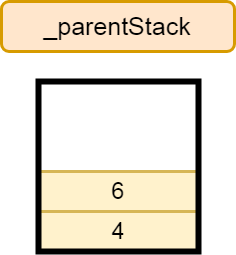
\includegraphics[width=0.2\textwidth]{Parser_AddingParentRelationToPKB.png}
\end{figure}
\textbf{Calls Relation
:} To add calls relation to PKB, the Parser will need to know the current procedure being parsed at all times. Hence, the Parser has a private attribute to store this information. When parsing a procedure call statement, the Parser validates the name of the procedure being called, and adds to PKB a call relation between the current procedure and the called procedure.\newline
\textbf{Next Relation
:} The Parser maintains a few data structures to add Next relation in PKB: 
\begin{enumerate}
\item Two boolean variables to indicate whether the current statement is just outside a while statement or an if-else statement. These two variables are named \_justExitIfElseStmt and \_justExitWhileStmt respectively.
\item Two stacks to keep track of nested while statements and if-else statements respectively. These stacks are named \_whileStmtStack and \_ifElseStmtStack respectively.
\item An unordered\_map<int, pair<int, int> > called \_ifElseStmtExitPoints to store the mapping of if-else statements to the exit points of if-else statements.
\end{enumerate}
\begin{center}
\fbox{\begin{minipage}{35em}
\texttt{procedure ABC \{
\newline1 \hspace{3mm}	a = 1;
\newline2 \hspace{3mm}	b = 2;
\newline3 \hspace{3mm} while x \{
\newline4 \hspace{12mm}  c = 4;
\newline5 \hspace{12mm}		if x then \{
\newline6	\hspace{21mm}	i = 6;
\newline \phantom{h} \hspace{12mm}	\} else \{ 
\newline7 \hspace{21mm} j= 7;
\newline \phantom{h} \hspace{11mm} \}
\newline8 \hspace{12mm}  k = 8;
\newline \phantom{h} \hspace{3mm} \}
\newline9 \hspace{3mm} m = 9;
\newline \}}
\end{minipage}}
\end{center}
\vspace{10mm}
Whenever the Parser adds the Follows relation in PKB as described earlier, it also adds the Next relation.

When the Parser encounters an if-else statement, the statement number is pushed onto the \_ifElseStmtStack. An integer variable is then used to store the if-else statement number for later use. When parsing the first statement in the if-block, the Parser will set Next relation for the if-else statement number and the first statement in the if-block. The Parser then continues to parse as usual until it reaches the last statement in the if-block. Now, the Parser uses another int variable to store the last statement in the if-block, then continues parsing until it reaches the first statement in the else-block. Here, the parser will set Next relation for the if-statement number and the first statement in the else-block. Before exiting the else-block, the Parser uses another int variable to store the last statement of the else-block, and push an element with the if-else statement number mapped to the last statement of the if-block and else-block into \_ifElseStmtExitPoints. The parser also sets \_justExitIfElseStmt to true, and then exits the else block. After exiting the else-block, if there is a statement encountered, the Parser will refer to \_ifElseStmtExitPoints to set Next relation for the statements:
\begin{enumerate}
\item The last statement of the if-block and the statement outside
\item The last statement of the else-block and the statement outside
\end{enumerate}
The top element of the \_justExitIfElseStmt and \_ifElseStmtStack are then popped and the variable \_justExitIfElseStmt is set back to false. \newline
When encountering a while statement, the statement number will be pushed onto the \_whileStmtStack. When parsing the first statement in the while-block, the Parser will set Next relation for the while statement number and the first statement in the while-block. The Parser then continues parsing until it reaches the last statement in the while-block. The Parser then add Next relation for the last statement in the while-block and the while statement. At this point, the \_justExitWhileStmt variable is also set to true. After exiting the while-block, if there is a statement encountered, the Parser will refer to the \_whileStmtStack to set the Next relation for the while statement and the statement just after the while-block. The top element of the \_whileStmtStack is then popped and the boolean variable \_justExitWhileStmt is set back to false. \newline
For the above code, when parsing statement 8, the data structures that Parser maintains is shown in Figure 4.
\begin{figure}[htbp]
  \caption{Keeping Track of Information of If-Else Statement to Add Next Relations
}
  \centering
    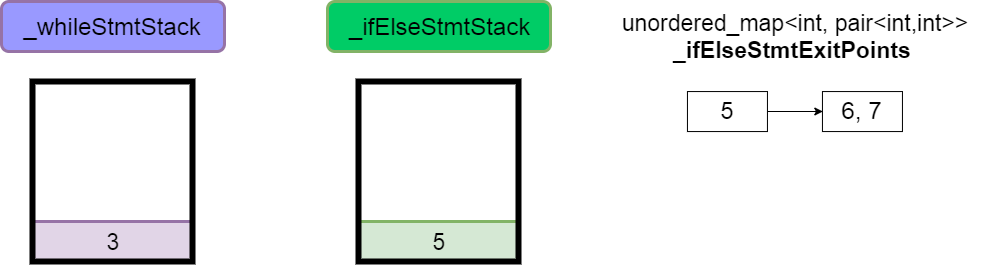
\includegraphics[width=0.85\textwidth]{Parser_AddNextRelationToPKB.png}
\end{figure}
\subsubsection{PKB}
Program Knowledge Base (PKB) provides a storage to store program design abstractions such as Uses, Modifies and other relations. Table-driven approach is used for the design of the PKB structure. Not only does it provides a simple yet powerful way to achieve flexibility, but it also allow quick accessing of the data by the way of hash maps. It has been decided that different class table files are made according to the different design entities. This is to make extension to allow additions of new design entities easier and this could minimize modifications of code.
\newline \textbf{\underline{Tables vs AST}}
\newline Abstract Syntax Tree (AST) is one of the conventional ways to store parsed data. However, when  the QueryEvaluator accesses data, it will have to perform tree traversal, which could take a lot of runtime during query processing and is not an optimal way. Also, doing modifications to allow more design entities would be more complicated. Alternatively, hash maps can be used to store data. Having multiple hashmaps over AST allows faster searching, addition, deletion of data.
\newline Hence, tables (in the form of hash maps) are used in this project so that query processing is done optimally in O(1) time. \newline
PKB contains the following components:
\begin{itemize}
\item PKB main 
\item Procedure Index Table
\item Variable Index Table
\item Statement Type Lists
\item Pattern Table
\item Follows/Follows* Table
\item Parents/Parent* Table
\item Uses Table
\item Modifies Table
\item Calls/Calls* Table
\item Next/Cache Table for Next*

\end{itemize}

\textbf{PKB-Main:} PKB-Main controls and stores all the tables in the entire PKB component, it will be used by only SPA front-end parser and query evaluator components in order to reduce coupling. The APIs of the PKB-Main plays a central role in the SPA architecture. \textbf{\underline{Procedure Index Table}}
\newline The Procedure Index Table stores all the procedures and their respective indexes. Before the parser starts parsing the SIMPLE source code, the procedure index is initialized to an arbitrary value of 0. Whenever a new procedure is added to its table by the parser, an index will be generated by the Procedure Index Table and used as a key for the procedure name.
Its structure is as follows:\newline
\underline{ProcIdxTable.h
}
\begin{itemize}
\item unordered\_map<string procName, int procIndex> procIdxMap
\item unordered\_map<int procIndex, string procName> procNameMap
\item int procIdx (initialized to 0, to generate indexes for procedures)
\end{itemize}
\textbf{\underline{Variable Index Table
}}
\newline The Variable Index Table is stored similarly as the Procedure Index Table.
Its structure is as follows:
\newline
\underline{VarIdxTable.h}
\begin{itemize}
\item unordered\_map<string varName, int varIndex> varIdxMap
\item unordered\_map<int varIndex, string varName> varNameMap
\item int varIdx (initialized to 0, to generate indexes for indexes)
\end{itemize}
\textbf{\underline{Statement Type List
}}
\newline The Statement Type List stores all the statement numbers added by the Parser, according to the respective entities. For example, if the statement number is an assignment statement, it is stored in the \textbf{assignList}. Similarly, statement number of the while statement is stored in \textbf{whileList}.  As such, when QueryEvaluator asks for assign or while statements, we are able to either retrieve the statement numbers that belong to a requested entity by filtering away unwanted data.
\newline Its structure is as follows: \vspace{10mm}\newline
\underline{StmtTypeList.h}
\begin{itemize}
\item list<int> allStmtList, to store statement numbers with entity ‘STMT’
\item list<int> assignStmtList, to store statement numbers with entity ‘ASSIGN’
\item list<int> whileStmtList, to store statement numbers with entity ‘WHILE’
\item list<int> ifStmtList, to store statement numbers with entity ‘IF’
\item list<int> callsStmtList, to store statement numbers with entity ‘CALLS’
\end{itemize}
\textbf{\underline{Uses Table
}}
\newline The Uses Table stores all the Uses relationships extracted by the Parser in the form hash maps (UsesTableStmtToVar) where the integer statement number or integer procedure index are keys, and a list of integer variable indexes are values. Firstly, when the design abstraction for Uses is added by the parser, the raw variable (or procedure) input in the form of string is converted to a variable (or procedure) index. Both the statement number and resultant integer index is then added to the hash map. Additionally, PKB also adds the reverse relationship internally to another hash map called UsesTableVar, where integer variable (or procedure) indexes as stored as a key, and statement numbers as a value. In the file UsesTableVar, it contains multiple maps such that the design abstraction can be stored according to the entity of the statement, so as to facilitate retrieval when queries such as Uses(a,v) and Uses(w, v) are called by the QueryEvaluator. \newline
\underline{UsesTableStmtToVar.h}
\begin{itemize}
\item unordered\_map<int stmtNum, list<int varIdx> > usesStmtToVarMap
\end{itemize}
\underline{UsesTableProcToVar.h}
\begin{itemize}
\item unordered\_map<int procIdx, list<int varIdx> > usesProcToVarMap
\end{itemize}
\underline{UsesTableVar.h}
\begin{itemize}
\item unordered\_map<int varIdx, list<int stmtNum> > usesVarToStmtMap
\item unordered\_map<int varIdx, list<int assignNum> > usesVarToAssignMap
\item unordered\_map<int varIdx, list<int procIdx> > usesVarToProcMap
\item unordered\_map<int varIdx, list<int whileStmtNum> > usesVarToWhileStmtMap
\item unordered\_map<int varIdx, list<int ifStmtNum> > usesVarToIfMap
\end{itemize}
\textbf{\underline{Modifies Table
}}
\newline The Modifies Table is populated similar to the Uses Table. \newline
\underline{ModTableStmtToVar.h}
\begin{itemize}
\item unordered\_map<int stmtNum, list<int varIdx> > modStmtToVarMap
\end{itemize}
\underline{ModTableProcToVar.h}
\begin{itemize}
\item unordered\_map<int procIdx, list<int varIdx> > modProcToVarMap
\end{itemize}
\underline{ModTableVar.h}
\begin{itemize}
\item unordered\_map<int varIdx, list<int stmtNum> > modVarToStmtMap
\item unordered\_map<int varIdx, list<int assignNum> > modVarToAssignMap
\item unordered\_map<int varIdx, list<int procIdx> > modVarToProcMap
\item unordered\_map<int varIdx, list<int whileStmtNum> > modVarToWhileStmtMap
\item unordered\_map<int varIdx, list<int ifStmtNum> > modVarToIfMap
\end{itemize}
\textbf{\underline{Pattern Table
}}
\newline The Pattern Table stores the patterns of all assignment, while, and if statements extracted by the parser. The pattern is stored as follows:\newline
\textbf{Key }- statement number in the form of integer.\newline
\textbf{Value} - a pair containing LHS variable and a postfix expression of the RHS in that statement number. \newline
When the pattern is added by the parser, the LHS variable is stored as a variable index with a type integer, whereas for the RHS expression, the raw input in the form of infix expression is computed internally into postfix by the Pattern Table. The first argument of pattern while and pattern if clauses are defined as control variables. This table will be accessed when pattern clauses are called by the query evaluator. Postfix is used in this table instead of infix in order to facilitate partial matching of the subexpression. \newline (E.g. 
Given an infix expression “a+b*(c-d)”, based on the rule of query evaluation, subexpression “c-d” partially matches using postfix, however, “a+b” does not, even though both expressions are the substrings of “a+b*(c-d)”. Hence partial matching is processed as shown:
“a+b*(c-d)” is converted to list(“a”,”b”,”c”,”d”,”-”,”*”,”+”)
The subexpressions “c-d” and “a+b” are also converted to list(“c”,”d”,”-”) and list(“a”,”b”,”+”) respectively.
list(“c”,”d”,”-”) is the sublist of list(“a”,”b”,”c”,”d”,”-”,”*”,”+”), whereas list(“a”,”b”,”+”)
Hence it can be deduced that “c-d” is the sub-expression of “a+b*(c-d)”, whereas “a+b” is not) \newline The steps below show how the partial matching is processed in general.
\begin{enumerate}
\item Raw input in the form of infix sub-expressions are passed to the function called hasPartialMatch(stmt, expression)
\item Within the function, the infix sub-expression is converted to postfix.
\item The postfix sub-expression performs the partial match by checking with the stored expression (postfix) that is retrieved from the pattern table.
\item If both expressions match, the function returns true.
\end{enumerate}
The structure is as follows:
\begin{itemize}
\item unordered\_map<int stmtNum, pair<int LHS, list<string> RHSexpression> > assignPatternTableMap
\item unordered\_map<int stmtNum, pair<int LHS, int controlVar> > whilePatternTableMap
\item unordered\_map<int stmtNum, pair<int LHS, int controlVar> > ifPatternTableMap
\end{itemize}
\textbf{\underline{Follows/Follows* table}}
\newline The Follows and Follows* Tables store all the Follows and Follows* relationships respectively. When the design abstraction Follows are parsed by the Parser, it adds the the statement number as a key, and the statements the current statement follows as a value (in the form of a pair<followedBy, follows>). Follows* relationships are then computed by the Design Extractor The table will be accessed when Follows(s1,s2) and Follows*(s1,s2) are called by the query evaluator. The structure is as follows: \newline
{\underline{FollowsTable.h}
\begin{itemize}
\item unordered\_map<int stmtNum, pair<int followedBy, int follows> > followsMap
\end{itemize}
{\underline{FollowsStarBefore.h}
\begin{itemize}
\item unordered\_map<int stmtNum, list<int> followedBy> followsStarBefore;
\end{itemize}
{\underline{FollowsStarAfter.h}
\begin{itemize}
\item unordered\_map<int stmtNum, list<int> follows> followsStarAfter;
\end{itemize}
\textbf{\underline{Parent/Parent* table}}
\newline The Parent and Parent* Tables store all the Parent and Parent* relationships respectively. When the design abstraction Parent is added by the Parser, the statement number is added to the hash map as a key, and the list of its children of its respective statements is added as a value. A reverse version of the hash map is implemented, so as to allow computation of the parent statement of the input. Parent* relationship is then computed by the Design Extractor. The table will be accessed when Parent(s1,s2) and Parent*(s1,s2) are called by the query evaluator. The structure is as follows: \newline
{\underline{ParentToChildTable.h}
\begin{itemize}
\item unordered\_map<int parent, list<int> children> parentToChildMap
\end{itemize}
{\underline{ChildToParentTable.h}
\begin{itemize}
\item unordered\_map<int child, int parent> childToParentMap
\end{itemize}
{\underline{ParentToChildStarTable.h}
\begin{itemize}
\item unordered\_map<int parent, list<int> children> parentToChildStarMap
\end{itemize}
{\underline{ChildToParentStarTable.h}
\begin{itemize}
\item unordered\_map<int child, list<int> parents> childToParentStarMap
\end{itemize}
\textbf{\underline{Calls/Calls* table}}
\newline The Calls and Calls* Tables store all the Calls and Calls* relationships respectively. It also stores the mapping of procedures as that is needed to compute transitive closures of Uses and Modifies relationships. Calls* relationship is then computed by the Design Extractor. The structure is as follows: \newline
{\underline{CallsTable.h}
\begin{itemize}
\item unordered\_map<int, list<int> > callsProcMap
\item unordered\_map<int, list<int> > callsProcMapReverse
\end{itemize}
{\underline{CallsStarTable.h}
\begin{itemize}
\item unordered\_map<int, list<int> > callsStarProcMap
\item unordered\_map<int, list<int> > callsStarProcMapReverse
\end{itemize}
\textbf{\underline{NextTable and Next* Cache}}
\newline The Next Table stores all the Next relations. It also acts as an adjacency list for the control flow graph which will be used for the computation of Next* relations in the Design Extractor. The Next* Cache stores all the Next* relations that were previously computed by PQL. This is to save time when retrieving identical Next* queries instead of recomputing them. The Next* Cache is only used within NextTable.h.
\newline
{\underline{NextTable.h}
\begin{itemize}
\item unordered\_map<int, list<int> > nextMap
\item unordered\_map<int, list<int> > nextMapReverse
\item NextStarCache NextStarCache
\end{itemize}
{\underline{NextStarCache.h}
\begin{itemize}
\item unordered\_map<int, list<int> > nextStarMap
\item unordered\_map<int, list<int> > nextStarMapReverse
\end{itemize}
\subsubsection{Design Extractor}} 
The role of the Design Extractor is to compute the complex relations from the tables that Parser has populated. It computes Parent*, Follows* and Calls* relations as well as the interprocedural Uses/Modifies relations. The Parser will call upon the Design Extractor to process these relations once it is done with parsing the SIMPLE source code. \vspace{4mm}\newline
\textbf{\underline{Computation of Parent*/Follows*/Calls* relations}}\newline
The computation of these complex relations are relatively similar and use the same algorithm. The Design Extractor iterates through the respective base tables (e.g. ParentsTable, FollowsTable) and appends the information found in these tables to the current list.
\begin{figure}[htbp]
  \caption{Parent to Child/ChildStar Table}
  \centering  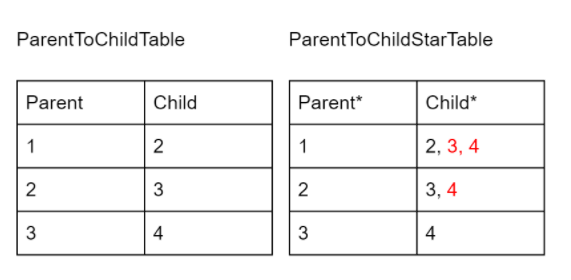
\includegraphics[width=0.7\textwidth]{ParentTable1.png}
\end{figure}
Using the computation of Parent* relations from the Parent relations table given in Fig.4 as an example, starting from statement 1, as the relation Parent(1, 2) is true, we then check if statement 2 is a parent statement. In this case, Parents(2, 3) exists, so 3 is appended onto the list of Child* in the ParentToChildStarTable[1]. We then continue to check the child of the current statement (in this case, statement 2) to see if it has a child statement. Since the relation Parent(3, 4) exists, we continue to append 4 onto ParentToChildStarTable[1]. Next, we check if statement 4 is a parent of any statement. Since there does not exist a child with statement 4 as its parent, all the Children* relationship for statement 1 has been computed. We then continue the same steps for all Parents in the ParentToChildTable. \newline
\begin{figure}[htbp]
  \caption{Child to Parent/ParentStar Table}
  \centering  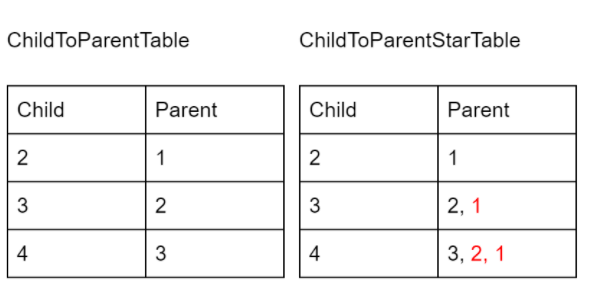
\includegraphics[width=0.7\textwidth]{ParentTable2.png}
\end{figure}
\vspace{4mm}
The reverse relations e.g. ChildToParentStarTable given in Fig.5 is also computed in the Design Extractor to facilitate faster result selection.

Similar to Parent and Parent* relations, Follows/Follows* and Calls/Calls* relations can be computed in the same manner.

\textbf{\underline{Computation of Inter-Procedural Uses/Modifies}}\newline
Computing Uses and Modifies relations that involve procedures requires a traversal of the Calls graph. Our Calls graph is essentially the table of Calls relationship, which acts as an adjacency list.The Design Extractor does a depth first search to reach the leaf nodes and propagate upwards in post-order fashion.
The Design Extractor iterates through every Caller procedure and starts a DFS from it. In a Calls graph, the arrow is directed from a Caller to a Callee (i.e. Calls(A, B)). 
\newline In this example, we will start the DFS from procedure A. 
\begin{figure}[htbp]
  \caption{Call Traversal from Proc A}
  \centering  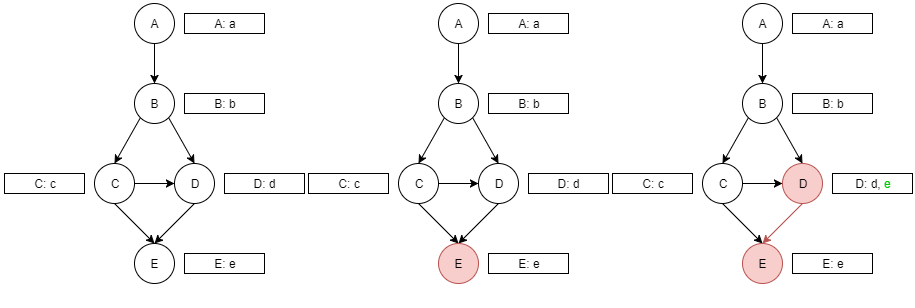
\includegraphics[width=1.0\textwidth]{Call_Traversal.png}
 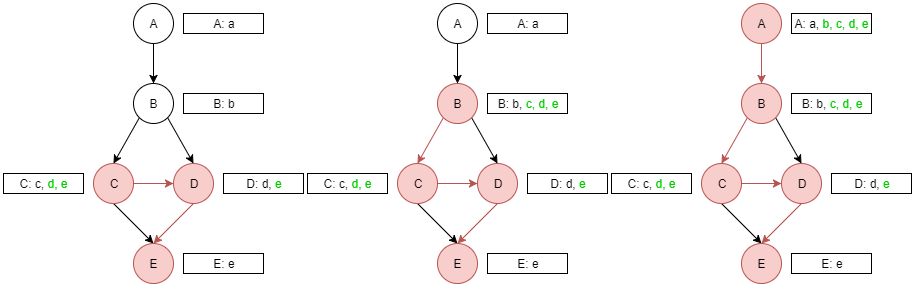
\includegraphics[width=1.0\textwidth]{Call_Traversal_2.png}
\end{figure}
\vspace{4mm}
From A, it will traverse down until procedure E and mark it as visited (highlighted in red). As E is a leaf node, it means that it does not call any procedures hence there are no new additional variables appended to its list of variables used. Once visited, it will reverse back to it’s parent, in this case procedure D. The Design Extractor then checks if all the procedures called by D have been visited. In this case, it is only E that is visited, and hence it appends the variables that E uses onto its list of variables used (in green).

From D, it returns back to its caller C. C checks if all its callees have been visited and if so, appends their used variables onto its list. If its callee’s nodes are not visited yet, we run the DFS on the callee. We do so until we return to node A, the node that we started with for this example.

The reason why this algorithm is run on every caller procedure is to ensure complete coverage of all Uses in the case where there could be multiple disjoint calls graphs. The same algorithm is run to compute inter-procedural Modifies relations.
\vspace{4mm}\newline
\textbf{\underline{Computation of Container Statement Uses/Modifies}}\newline
After the population of inter-procedural modifies relations, we can then compute Uses and Modifies relations for container statements that contain a call statement in their statement list.

The Design Extractor will retrieve all the Call statements and find the list of Parent* of it. For each Parent*, it will sent that Parent*’s statement to use the variables that are used by the procedure of the Call statement. \newline Consider the following source code
\begin{center}
\fbox{\begin{minipage}{35em}
\texttt{procedure A \{
\newline1 \hspace{3mm}	while a \{
\newline2 \hspace{10mm}	while c \{
\newline3 \hspace{17mm} call B;
\newline \hphantom{he} \hspace{15mm} \}
\newline \hphantom{he} \hspace{7mm}		\}
\newline 	\}
\newline procedure B \{
\newline4 \hspace{3mm}  x = a + b + c;
\newline \}}
\end{minipage}}
\end{center}
\vspace{10mm}
The Design Extractor will get the list of call statements, in this case only statement number 3. Then, it will get all the Parent* of statement 3 which are {2, 1}. For all the Parent* statements, {2, 1}, their use relations would be updated with the variables used by statement 3, {a, b, c}.
\begin{figure}[htbp]
  \caption{Statement to Variable Tables}
  \centering  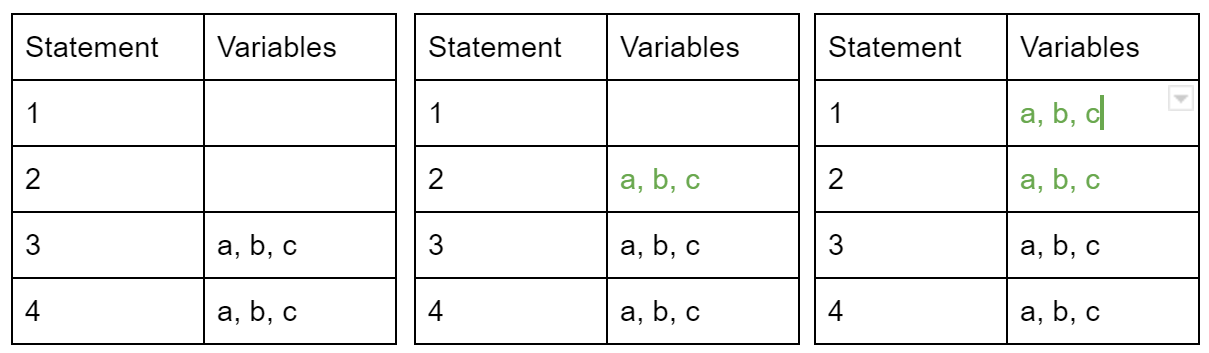
\includegraphics[width=1.0\textwidth]{uses_propagating.png}
\end{figure}
\vspace{4mm}

The same idea used in computing Uses relation and Modifies relation for container statements.

\subsubsection{PQLMain}
The PQLMain is the main class that other components interact with. PQLMain employs the \textbf{Facade} pattern, whereby other components that need to use PQLMain do not need to know the implementations and the sub-components inside PQLMain. When it is initialised, it takes in a query string and instantiates a blank QueryTree (the main storage component) which is used throughout the process of  query processing and evaluation. Fig.7 shows the component diagram of the PQLMain and its sub-components. \newline
\begin{figure}[htbp]
  \caption{PQLMain Facade Component diagram}
  \centering 
 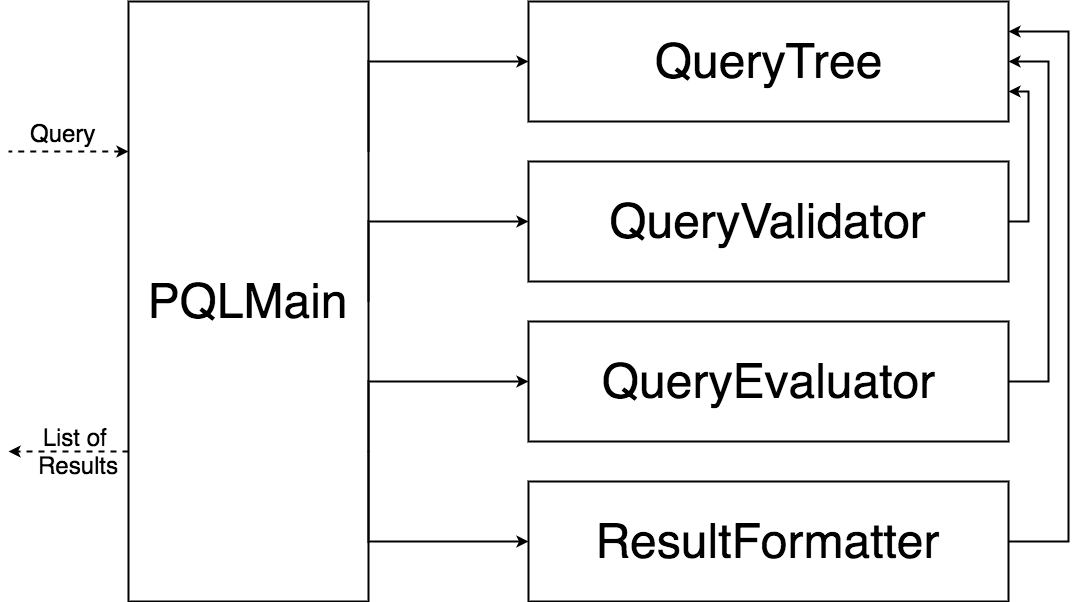
\includegraphics[width=0.7\textwidth]{PQL_Main.png}
\end{figure}
\subsubsection{Query Validator}
The QueryValidator ensures that the query received from PQLMain is syntactically and semantically correct. A series of validation steps are executed while parsing the query to check whether the structure of the query is well-formed and whether the arguments of each individual clause are declared and consist of permitted argument types as described in the program design model. It relies heavily on regular expressions (Regex) that are aligned to the PQL grammar. As the QueryValidator performs its validation routine, it also helps to build an internal storage structure, the QueryTree, by storing only essential parts of the query. This watered-down version of the query will ease the work of the QueryEvaluator. \newline
The steps parsing the query given below are as follows:
\begin{center}
\fbox{\begin{minipage}{40em}
\begin{flushleft}stmt s; assign a, a1  , a2;
\newline Select s such that Follows (s, a) pattern a(\_, \_) with a.stmt\# = s.stmt\#
\end{flushleft}
\end{minipage}}
\end{center}
\vspace{4mm}
\begin{enumerate}
\item Upon receiving a query from PQLMain, the QueryValidator will attempt to dissect the query into Declaration and Selection. This can be done by splitting the query with semi-colons as the delimiter. As each valid query will have its Selection as the last token, any token before the last will be considered as Declaration.
\begin{figure}[htbp]
  \caption{State of query after dissection}
  \centering 
 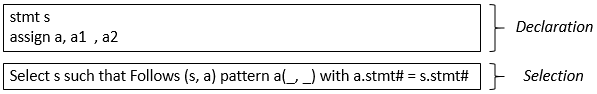
\includegraphics[width=1.0\textwidth]{DissectedQuery.png}
\end{figure}
\item The QueryValidator will first process each token in Declaration. Each token is further split it into sub-tokens using whitespace as the delimiter.
\begin{figure}[htbp]
  \centering 
 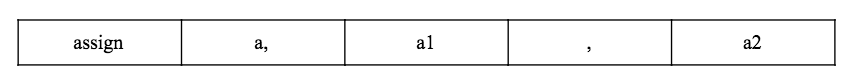
\includegraphics[width=1.0\textwidth]{Step2.png}
\end{figure}
The first sub-token will be compared against the acceptable entity as defined in the PQL grammar. If it is invalid, the QueryValidator will immediately return false. If it is valid, it proceeds, and for all subsequent sub-tokens, if any of them are invalid, the QueryValidator will return false. Otherwise, the QueryValidator will count the number of commas in all the declaration statements and compare them with the expected number of commas. One observation made by the team was that the difference between the number of commas and the sum of entity and synonyms is 2. Using this fact, the QueryValidator finishes validation for multiple declarations of the same entity type. For every valid synonym recognized, the QueryValidator inserts it, together with the entity,into the QueryTree. For the above example, the expected number of commas is 2 and the sum of entity and synonyms is 4.
\item After processing Declaration, the QueryValidator will compare Selection against the overall regex definition derived from the PQL grammar. This regex picks up clause group as shown below
\begin{figure}[htbp]
  \centering 
 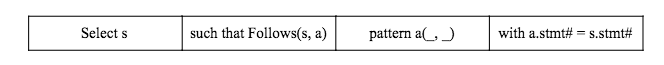
\includegraphics[width=1.0\textwidth]{Step3.png}
\end{figure}
\item With the query being partitioned into distinctive clauses, the QueryValidator validates each clause independently. For each clause, the QueryValidator passes it to SelectionValidator. As the query has already passed the overall regex check, there is no need to look for clause keywords to determine which clause they belong to, hence clause keywords (‘select’, ‘such that’, ‘pattern’, ‘with’ and ‘and’) can be dropped.
\begin{figure}[htbp]
  \centering 
  \caption{QueryValidator Selection: State of clause before SelectionValidator passes it to the respective handlers}
 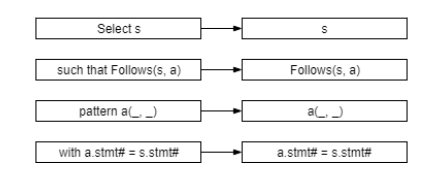
\includegraphics[width=0.7\textwidth]{ClauseState.png}
\end{figure}
\end{enumerate}
The SelectionValidator will then pass the processed clause to the respective clause handler that is supposed to handle that type of clause. The Handler will then delegate the respective sub-validators to validate and extract the arguments and types of argument. The Handlers adopts the \textbf{Strategy} pattern to determine which sub-validator to pass the clause to.
\begin{figure}[htbp]
  \centering 
  \caption{QueryValidator Handler: Possible path taken}
 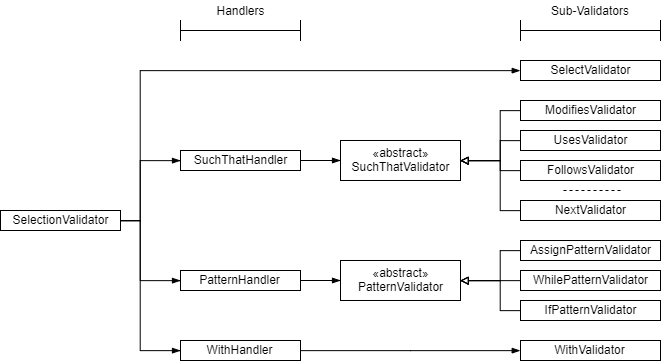
\includegraphics[width=1.0\textwidth]{QVHandler.png}
\end{figure}
Each sub-validator extracts the argument and enquires the QueryTree for the type of argument. Once the sub-validator receives the information from the QueryTree, it will tag each argument to its appropriate type.

Arguments are tagged according to their entity type, specific to their respective clauses. The tagging system makes use of enums. \newline
\begin{comment}
\begin{table}
\centering
\begin{tabular}{|c|c|}
\hline
\cellcolor{green!35}Enum Relationship & \cellcolor{green!35}Value \\\hline
MODIFIES & 0 \\\hline
USES & 1 \\\hline
PARENTS & 2 \\\hline
PARENTSTAR & 2 \\\hline
FOLLOWS & 3 \\\hline
FOLLOWSSTAR & 4 \\\hline
CALLS & 5 \\\hline
CALLSSTAR & 6 \\\hline
NEXT & 7 \\\hline
NEXTSTAR & 8 \\\hline
AFFECTS & 10 \\\hline
AFFECTSSTAR & 11  \\\hline
\end{tabular}
\caption{\label{Relationship Enum}
\end{table}
\begin{table}[htbp]
  \caption{Entity Enum}
 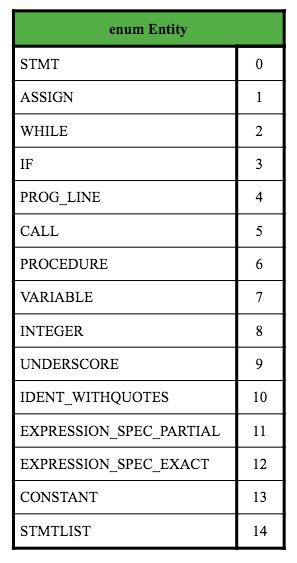
\includegraphics[width=0.3\textwidth]{EnumEntity.png}
\end{table}
\end{comment}
\begin{table}[htbp]
  \caption{Relationship Enum}
 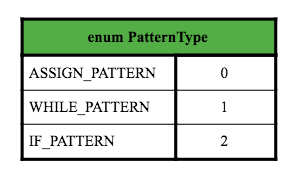
\includegraphics[width=0.3\textwidth]{Pattern_Enum.png}
 \end{table}
\begin{table}[htbp]
  \caption{Pattern Enum}
 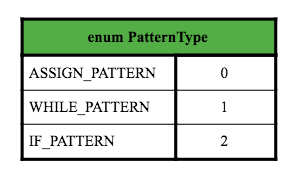
\includegraphics[width=0.3\textwidth]
{Pattern_Enum.png}
 \end{table}
\begin{table}[htbp]
  \caption{Attribute Enum}
 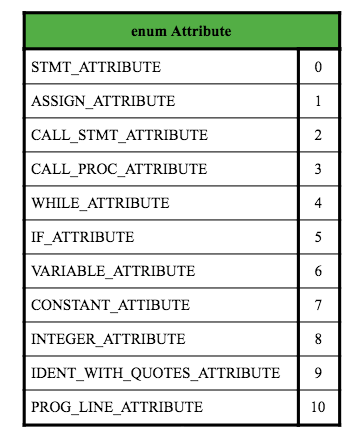
\includegraphics[width=0.3\textwidth]{Attribute_Enum.png}
\end{table}
\newline Upon validation and extraction, the sub-validators will return their results to the Handler. The generation of ClauseObject is done via the Factory pattern, using the information retrieved from each sub-validatos. Handler will encapsulate this information into a ClauseObject before storing it in the QueryTree.
\begin{figure}[htbp]
  \centering 
  \caption{Query Validation Handler}
 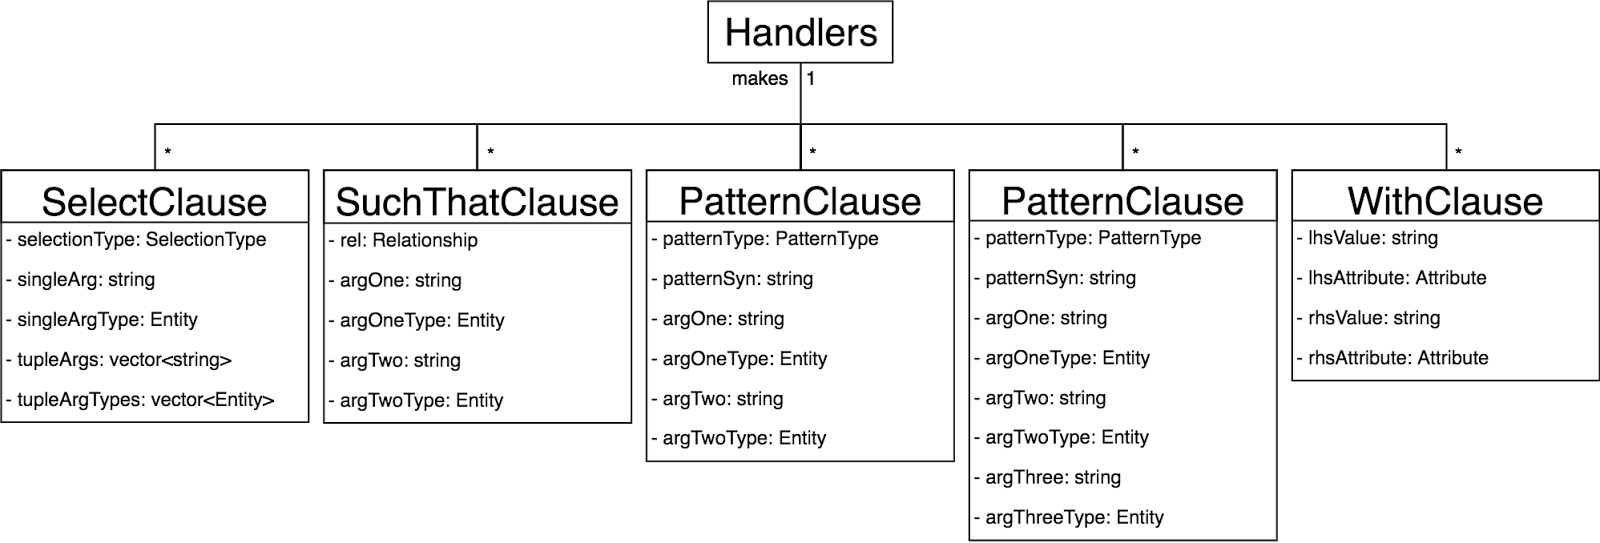
\includegraphics[width=1.0\textwidth]{ClauseInteraction.png}
\end{figure}
\begin{figure}[htbp]
  \centering 
  \caption{Validator Flowchart}
 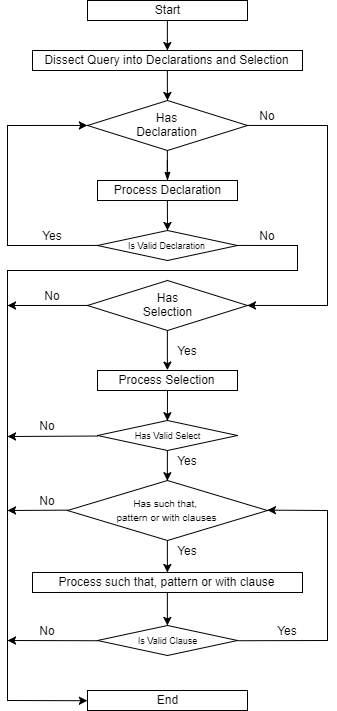
\includegraphics[width=0.5\textwidth]{ValidatorFlowchart.png}
\end{figure}

The decision making at each stage is shown in Fig. 12 above.
\subsubsection{Query Optimizer (plan)}
The QueryOptimizer will be designed to group the different clauses to get an optimal evaluation time in the QueryEvaluator. The QueryOptimizer will work on the query after finishing query validation and before starting evaluation. 
The main heuristic for optimization is to avoid cross-products, which is a time consuming operation. Thus, the team’s tentative plan is to first group the different clauses according to the following rules:-

\textbf{Group 0:} Clauses that return boolean results (e.g Follows(1,2), Uses(1,“x”)) \newline
\textbf{Group 1:} Clauses containing synonyms that are not required by the Select clause (e.g Select s such that Follows(s,s1) and Follows(s3,s4) will put Follows(s3,s4) in Group 1) \newline
\textbf{Group 2:} Clauses containing synonyms required by the Select clause for intermediate results.

For 'with' clauses, the QueryOptimizer will implement overwriting of clauses (e.g if the query is 
procedure p; Select s such that Modifies(p,“x”) with p.procName = “Pikachu”, the such that clause that will be passed to the evaluator will be Modifies(“Pikachu”,“x”).

\subsubsection{Query Evaluator}
The QueryEvaluator is used to retrieve design entities from the PKB that fulfill query specifications. It first retrieves the Clause objects (created by the QueryValidator) from the QueryTree. For each Clause object, the QE will evaluate the clause with the help of appropriate ClauseEvaluators and proceed with the evaluation. These evaluators assist the QE in retrieving the relevant results from the PKB and are produced by providing Clause object to the ResultsFactory. We first discuss the intermediate data structures that we utilise, before providing an in-depth discussion of the evaluation steps taken by the QE.\newline
\textbf{ClauseResult} \newline
\begin{figure}[!htbp]
  \centering 
  \caption{ClauseResult}
 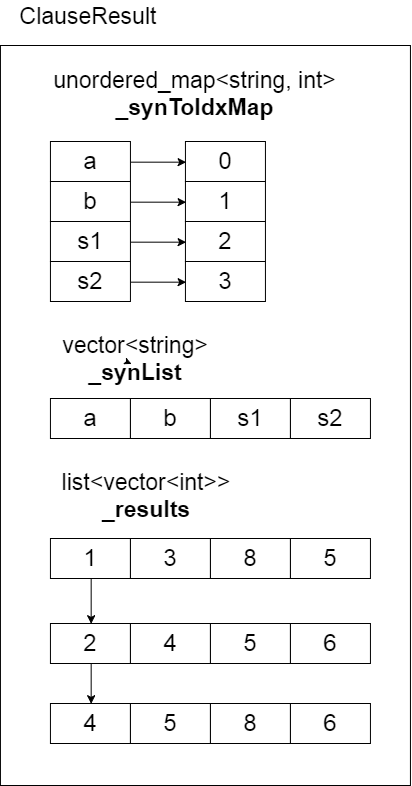
\includegraphics[width=0.3\textwidth]{ClauseResult.png}
\end{figure}
The ClauseResult is responsible for storing and maintaining the intermediate results across Clause objects as they are evaluated by the QueryEvaluator. The ClauseResult maintains several data structures to achieve this purpose.

The intermediate results are stored in a list<vector<int> > data structure, where each vector<int> represents one combination of all synonyms that satisfies the clauses evaluated so far. A vector is used to store these combinations because it allows access of the values of selected synonyms in O(1) time with indexing. This means that every index position in the vector is mapped to a certain synonym, and this mapping is the same for all vectors in the list. A list is used to store these vectors because combinations of synonym values will need to be inserted and removed from the middle of the list often, and a linked-list can carry out these operations in O(1).

As the index positions in the aforementioned vectors need to be mapped to synonyms, an unordered\_map<string, int> is used to store the mapping between synonyms and their indices, and a list<string> is used to implicitly store the reverse mapping.
\newline \textbf{Evaluation Process} \newline
The evaluation steps are listed below:

As per the \textbf{Strategy} pattern, each clause in the clause group will have an evaluator created specially for its evaluation. Figures 16,17 and 18 show an overview of the various evaluators, derived from the base class ResultEvaluator. 
\begin{enumerate}
\item When invoked, the evaluate method of the QE retrieves the vector of Clause objects from the QueryTree.
  
\item The QE then initialises the ResultFactory and feeds the Clause objects, one at a time, to the ResultFactory to be processed. The Clause objects will be processed in the order of SuchThatClause, PatternClause, followed by WithClause and lastly SelectClause. At any point, if one clause should return false due to invalid evaluation or all results get removed from the ClauseResult, the whole evaluation process will be discontinued.

\item As per Strategy pattern, the ResultFactory will create evaluators specially for the evaluation of the clauses. Figures 16,17 and 18 show the overview of the various evaluators that can be created. 
   \begin{center}
\begin{figure}[!htbp]
  \caption{With Evaluator}
 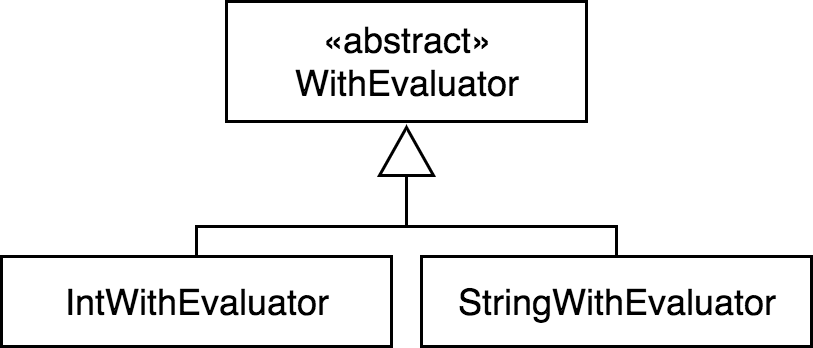
\includegraphics[width=0.5\textwidth]{WithEvaluator.png}
\end{figure}
\end{center}
\begin{figure}[!htbp]
  \centering 
  \caption{Pattern Evaluator}
 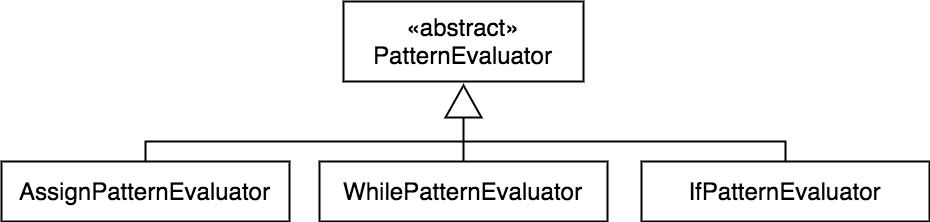
\includegraphics[width=0.8\textwidth]{PatternEvaluator.png}
\end{figure}
\begin{figure}[!htbp]
  \centering 
  \caption{Such That Evaluator}
 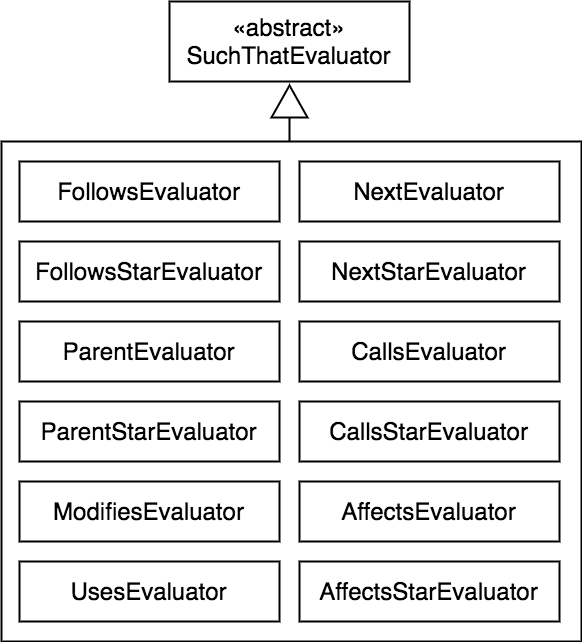
\includegraphics[width=0.5\textwidth]{SuchThatEvaluator.png}
\end{figure}
Generation of an evaluator is done via the Factory pattern, using the information retrieved from Clause objects. The appropriate evaluator is chosen based on the type reference of the Clause objects. For example, the SuchThatEvaluator has a relationship type specifier while the PatternEvaluator has a pattern type specifier.
\item Evaluators determine how to evaluate results by passing the arguments of a clause through several cases. Each clause will have its own cases to evaluate depending on the type of inputs that they allow. Table 5 shows an example of the evaluation cases for the Follows relationship.
\begin{table}[!htbp]
  \centering 
  \caption{Follows Evaluator Cases}
 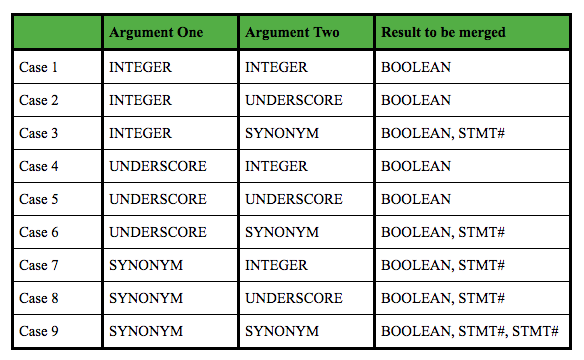
\includegraphics[width=0.8\textwidth]{FollowsEvaluatorCases.png}
\end{table}
\item After the specific evaluators evaluate the clauses, the results of the current clause will be merged into the ClauseResult object, which keeps track of the intermediate results. For purely  Boolean  cases (i.e. Follows(3, 4); Case 1 in Table 5), only the validity is returned by the evaluator, and this determines whether evaluation will proceed with the next clause. The validity replaces any previously stored boolean value. Recall that the evaluating process will be terminated if the stored validity is false; thus a false stored validity will never be overwritten . For cases with  Synonyms , the validity is returned,   and   results   are   stored   or   modified   in   the   ClauseResult   via   its   reference   pointer.
\item For clauses that contains synonyms, there are 5 possible cases that may arise.
\begin{table}[!htbp]
  \centering 
  \caption{Cases of Clauses with Synonyms}
 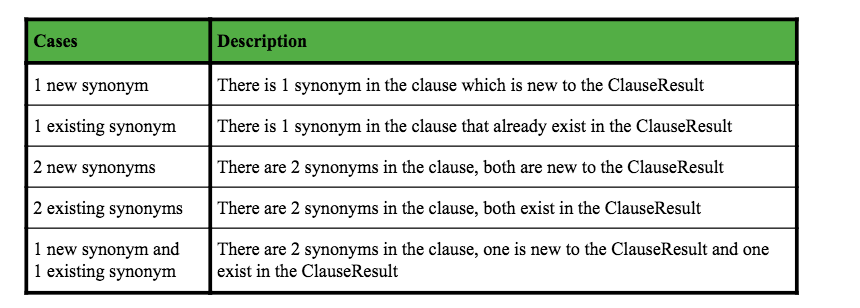
\includegraphics[width=1.0\textwidth]{SynonymClauses.png}
\end{table}
\newline For the cases of 1 new synonym and 2 new synonyms, the way the ClauseResult works depends on whether there are already other synonyms existing in the ClauseResult. These two scenarios are illustrated in the following diagram.
\begin{figure}[!htbp]
  \centering 
  \caption{Adding New Single Synonym Results}
 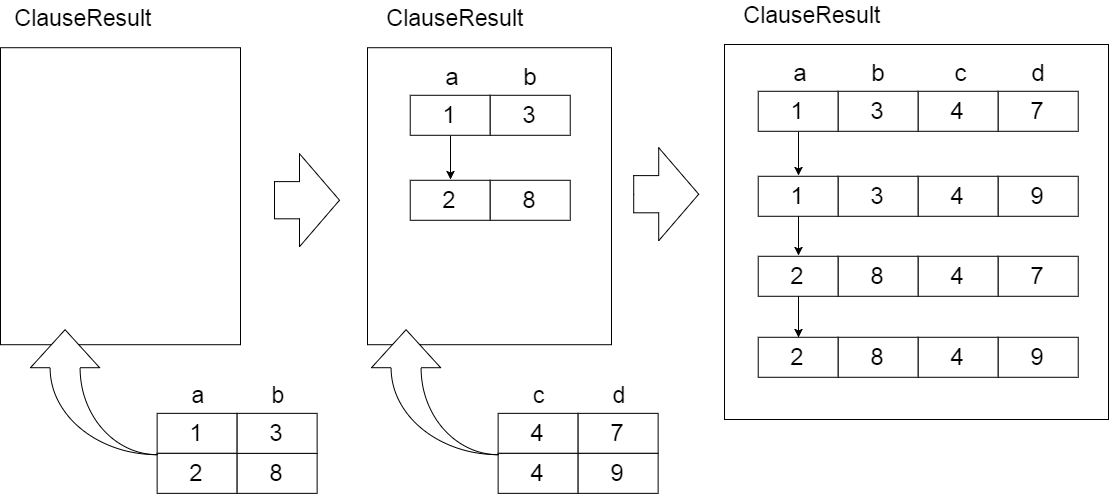
\includegraphics[width=0.8\textwidth]{ClauseResult_AddTwoNew.png}
\end{figure}
\newline Notice that for the case of 2 new synonyms, PKB will need to compute all pairs of the two synonyms for evaluator, which is an expensive process. Optimisation to avoid this scenario is possible, which will be introduced in future iterations. \newline For the cases of 1 existing synonym and 2 existing synonyms, the ClauseResult will loop through the existing results and remove the ones that do not have a match in the new result list
\begin{figure}[!htbp]
  \centering 
  \caption{Adding Existing Synonym Results}
 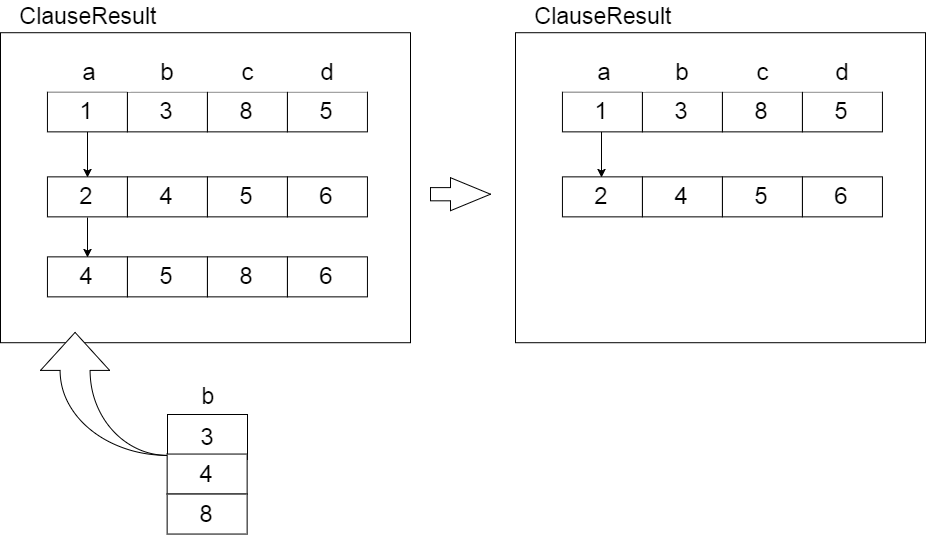
\includegraphics[width=0.8\textwidth]{ClauseResult_AddExistingSynonym.png}
\end{figure}For the case of 1 new synonym and 1 existing synonym, the ClauseResult 
\begin{figure}[!htbp]
  \centering 
  \caption{Adding A New Synonym Paired to an Existing Synonym}
 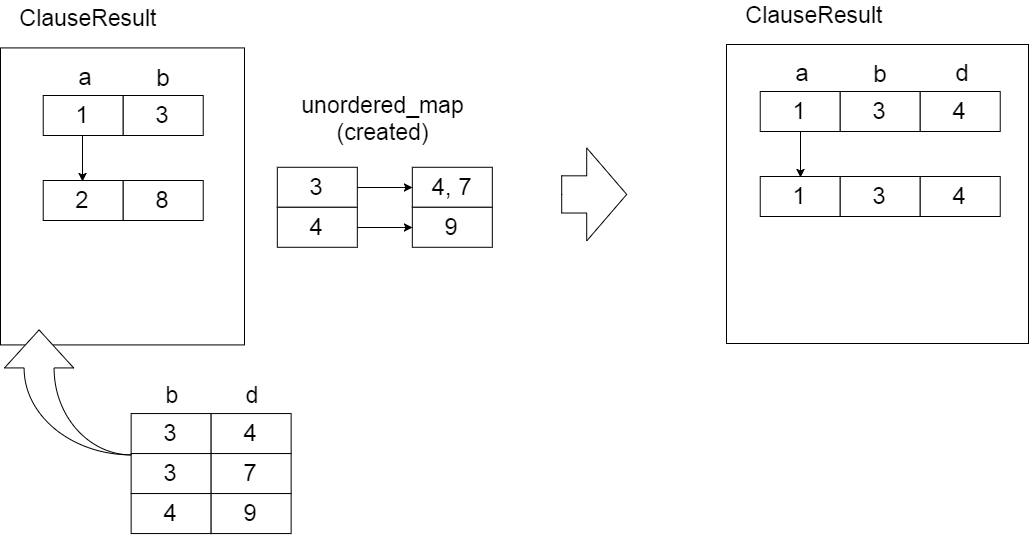
\includegraphics[width=0.8\textwidth]{ClauseResult_AddOneNewOneExisting.png}
\end{figure}
will create an unordered\_map<int, list<int> > to help with the merging process, this unordered\_map will map each values of the existing synonyms to the list of the corresponding values of the corresponding new synonym. For each of the existing result combination, if the common synonym’s value has a match in the unordered\_map, the new synonym’s value will be appended to the combination. If the common synonym’s value has no match in the unordered\_map, the combination will be discarded.

If the number of combinations of the existing results is M, and that of the results to merge is M, the time complexity of this merging process would be O(M+N), which is sufficiently fast.

\item After the ResultFactory has finished processing all the Clause objects and all of them returns true for validity, the factory will call the makeClauseResult() method to return the final ClauseResult object back to QE. QE will then store this back into the QueryTree, waiting for it to be picked up by the ResultFormatter to format and return the final result.

\end{enumerate}
\subsubsection{Result Formatter}
The ResultFormatter uses the QueryTree and the ClauseResult to return results in the form of a list of strings (list<string>)  back to the UI. It first checks the type of the Select clause (whether it’s BOOLEAN, single synonym or tuple). 
\begin{enumerate}
\item If the query selects BOOLEAN, the ResultFormatter checks whether the ClauseResult has results and if QueryTree has any clauses to evaluate. If QueryTree contains clauses to evaluate, if ClauseResult doesn’t have results after evaluation, then the ResultFormatter returns a ‘false’ result; it returns ‘true’ for all other cases.
\item If the query selects a single synonym/tuple, then ResultFormatter uses ClauseResult’s API getSynonymResults() to get the raw results. If the synonym being selected returns a numerical result, then the list of integers (list<int>) is converted to a list of strings (list<string>) and projected to the UI. In case the synonym being selected needs to return a string result (e.g entities of the type VARIABLE and PROCEDURE) the list of integers received from ClauseResult are converted to a list of strings according to the mapping done by PKB (as previously, we map all strings to ints to optimize Query Evaluator; thus, we need to convert the mapped ints to strings when we output the results)
\end{enumerate}
\subsection{Design decisions}
\subsubsection{Parsing Strategy}
\begin{tabular}{|L{5cm} | L{12cm}| }
\hline
Problem &
The Parser has a lot to do while parsing the SIMPLE source code:\newline
- Various types of syntax validation
\newline - Display error message as user feedback when syntax error is detected
\newline - Extract various design abstractions and populate PKB
 \\
    \hline
    Alternatives &
1. Do all of the job of the parser in one parse
\newline 2. Do many parses, each parse doing one particular task, e.g. bracket-matching, Calls relation, Uses relation, etc.
\newline 3. Hybrid of the above two alternatives. \\
\hline
    Criteria for comparison &
1. Time-efficiency
\newline 2. Ease of implementation
\newline 3. Testability
\newline 4. Maintainability
\newline 5. Extensibility to iteration 2, iteration 3, and possible bonus features 
 \\
 \hline
   Decision & \textbf{Choice: Hybrid}
\newline
Doing everything in one parse can be difficult to implement and error-prone. It also makes testing difficult. On the other extreme, having many parses, each doing one simple task will also result in a lot of duplicate codes, which will make parser difficult to be maintained and extended because if there is a need to change something, all the duplicated code will need to be changed.
\newline
Therefore, using just a few parses with each parse doing related tasks is probably the most reasonable design. The Parser will do one parse just to check whether braces are paired up correctly, and do a second parse to extract design abstractions and populate PKB.
 \\
 \hline
\end{tabular}
\subsubsection{PKB Design: Representation of Design Abstraction}
\begin{tabular}{|L{5cm} | L{12cm}| }
\hline
Problem &
Speed is a very important aspect for query evaluation. If this aspect is neglected, it would cause a longer runtime when multiple queries are processed. Therefore, design of the data structures to store and represent design abstractions added by the parser is extremely crucial to ensure that data is accessible at the shortest time possible.
 \\
    \hline
    Alternatives &
- AST
\newline - Tables in the form of hash maps
 \\
\hline
    Criteria for comparison &
1. Time complexity of retrieval, addition and deletion
\newline 2. Simplicity of implementation 
\newline 3. Extensibility to future iterations and possible bonus features
\newline 4. Testability
 \\
 \hline
   Decision & \textbf{Choice: Tables in the form of hash maps}
\newline
AST is the conventional ways to store parsed data into. However, when it comes to accessing the data by the Query Evaluator component, it has to perform traversing of the tree, which could take a lot of time during query processing. Also, doing modifications to allow more design entities would be more complicated. Alternatively, hash maps can be used to store data. Having multiple hashmaps rather than AST allows faster searching, addition, deletion of data. 
 \\
 \hline
\end{tabular}
\vspace{5mm}
The table below shows the time complexity of query processing when AST and tables are used. '$s$' represents the number of statements in the SIMPLE programme):
\begin{table}[htbp]
\begin{tabular}{|c|c|c|}
\hline
 & Using AST & Using Tables\\
\hline
Data searching & $O(log\hspace{1mm}s)$& $O(1)$\\
\hline
Retrieving single data & $O(log\hspace{1mm}s)$& $O(1)$ \\
\hline
Retrieving all the data & $O(s\hspace{1mm}log\hspace{1mm}s)$ & $O(s)$\\
\hline
\end{tabular}
\end{table}
\subsubsection{PKB Design: Evaluating reverse relationships}
\begin{tabular}{|L{5cm} | L{12cm}| }
\hline
Problem &
For queries that require retrieval of the left hand parameter (as in x in Uses(x,y), Modifies(x,y), etc.), the key of the hash map needs to be retrieved from the input value. For example, if the query evaluator calls Follows(3, s), statement s can be retrieved in $O(1)$ time, by using the key ‘3’. However, if Follows(s, 3) is called, since ‘s’ is an unknown key, it is not possible to retrieved in constant time. Therefore, traversing is needed to find the key that matches with the value, and it could take $O(n)$ time complexity at its worst.
 \\
    \hline
    Alternatives &
- Add another hash maps to store reverse relationships
\newline - Self-balancing binary search tree (BST) 
 \\
\hline
    Criteria for comparison &
1. Time complexity for retrieval
\newline 2. Ease of implementation
 \\
 \hline
   Decision & \textbf{Choice: Add another data structure to store reverse relationships}
\newline
The time complexity of searching in hash maps is faster compared to searching in trees, as traversing of trees takes $O(log n)$ time. A drawback in this method is that adding an extra data structure doubles the space complexity, but the priority of this SPA is the speed and efficiency of data retrieval, rather than the size of the program. Therefore, sacrificing memory space for better speed is more practical.
 \\
 \hline
\end{tabular}
\subsubsection{PKB Design: CFG Design}
\begin{tabular}{|L{5cm} | L{12cm}| }
\hline
Problem &
Storage of CFG
 \\
    \hline
    Alternatives &
- Adjacency List
\newline - Adjacency Matrix
\newline - Edge List

 \\
\hline
    Criteria for comparison &
1. Time complexity for finding relation
\newline 2. Time complexity for traversal
\newline 3. Ease of implementation
 \\
 \hline
   Decision & \textbf{Choice: Adjacency List}
\newline
Time complexity for finding relation: Edge List $O(E)$ > Adjacency List $O(2)$ = $O(1)$ = Adjacency Matrix $O(1)$. \newline
Time complexity for traversal: Edge List $O(E)$ > Adjacency Matrix $O(V^2)$ > Adjacency List $O(V)$ \newline
Time complexity for finding relation in Adjacency List in our CFG is $O(1)$ as each statement in the CFG can have at most 2 vertices. Therefore, Adjacency List is the best for retrieval of a relation as well as for graph traversal. At the same time, the way PKB stores next relations are already in an Adjacency List format. Hence it is easier to use the table of all next statements as our Adjacency List.

 \\
 \hline
\end{tabular}
\subsubsection{Pattern Matching: Representation of expressions}
\begin{tabular}{|L{5cm} | L{12cm}| }
\hline
Problem &
Pattern matching requires consideration of the precedence of operators and associativity, therefore it cannot be performed by matching substrings. Therefore, an alternate representation of expressions is required to facilitate pattern matching.
 \\
    \hline
    Alternatives &
- Trees to represent expression
\newline - Postfix matching


 \\
\hline
    Criteria for comparison &
1. Time complexity of retrieval
\newline 2. Simplicity of implementation
\newline 3. Testability
 \\
 \hline
   Decision & \textbf{Choice:  Postfix matching}
\newline
Postfix matching is used instead of trees due to the fact that trees are harder to implement and make debugging more time consuming. Postfix expressions can be represented in a list of strings containing operator/operands, and they can be easily inserted into and retrieved from hash maps. Pattern matching can be done by comparing sublists.
 \\
 \hline
\end{tabular}
\subsubsection{Query Validation Design}
\begin{tabular}{|L{5cm} | L{12cm}| }
\hline
Problem &
1. Difficulty in parsing query
\newline 2. Too many if-else string comparisons
 \\
    \hline
    Alternatives &
1. Usage of Regular Expression
\newline 2. Naive tokenizing with specific delimiter
\newline 3. Naive if-else
 \\
\hline
    Criteria for comparison &
1. Time-efficiency
\newline 2. Ease of implementation
\newline 3. Testability
\newline 4. Maintainability
\newline 5. Extensibility to iteration 2, iteration 3, and possible bonus features\\
 \hline
   Decision & \textbf{Choice:  Regular Expression}
\newline
Parsing the query may be tedious as there are many considerations to take into account to when choosing the delimiters. Regex provides a fast and elegant solution. One line of regex can replace a hundred lines of procedural code. As members of  the group are well-versed and experienced with regex, implementation was fast. Regex is easier to maintain, especially when they are stored in string constants that can be reused and concatenated to form a larger expression.
 \\
 \hline
\end{tabular}
\begin{tabular}{|L{5cm} | L{12cm}| }
\hline
\cellcolor{green!25}Problem &
Many “if-else” statements to handle the validation of clauses
 \\
    \hline
\cellcolor{green!25}Alternatives &
Strategy pattern (Handlers and sub-validators)
 \\
\hline
\cellcolor{green!25}Criteria for comparison &

\textbf{Pros} \newline
1. Easy modification and extension as understanding the individual strategy to process each clause does not require you to understand the entire process.
\newline 2. Less tedious to maintain and extend the code as changes only need to be done in a class design as compared to all classes.
\newline 3. Eliminates conditional statements for selecting the correct validator to process each clause. \newline

\textbf{Cons} \newline
1. Increase overhead in terms of memory space and execution time.
\newline 2. Increase number of classes to handle the validators.
\newline 3. Increase complexity of the solution.
\\
 \hline
\end{tabular}
\subsubsection{Query Evaluation Design}
\begin{tabular}{|L{5cm} | L{12cm}| }
\hline
\cellcolor{green!20}Problem &
Many “if-else” statements to handle the evaluation cases of all the clauses, deeply nested nested if else blocks makes extension of the evaluators very tedious
 \\
    \hline
\cellcolor{green!25}Alternatives &
1. Strategy pattern (ClauseEvaluator and sub-classes)
\newline 2. Factory pattern (ResultFactory and ClauseResult)
 \\
\hline
\cellcolor{green!25}Criteria for comparison &
\textbf{Pros: Strategy Pattern} \newline
1. Modifying or understanding the individual strategy to process each clause does not require you to understand the entire process.
\newline 2. Less tedious to maintain and extend the code as changes only need to be done in a class design as compared to all classes.
\newline 3. Eliminates many conditional statements for evaluator to select the correct function to process each clause. \newline
\textbf{Pros: Factory Pattern} \newline
1. Lazy initialization to delay creation of the subunit processors to process each clause. 
\newline 2. A single point of control to create the subunit processor, which are evaluators.\newline
\textbf{Cons} \newline
1. Increase overhead in terms of memory space and execution time.
\newline 2. Increase number of classes to handle the validators.
\newline 3. Increase complexity of the solution.
\\
 \hline
\end{tabular}
\subsubsection{Data Structures for Intermediate Result}
\begin{tabular}{|L{5cm} | L{12cm}| }
\hline
Problem &
The data structures of intermediate result is crucial for the good performance of PQL queries as numerous operations will need to be carried out on the intermediate result when evaluating each clauses. These operations include merging of tables, insertions, deletions, and many more, which might be computationally expensive if not optimised.
 \\
    \hline
    Alternatives & Representation of results: \newline
1. Actual form (e.g. integer for statement, string for variable/procedure names)
\newline 2. Indices \\
\hline
    Criteria for comparison &
1. Time-efficiency
\newline 2. Ease of implementation
\newline 3. Testability
\newline 4. Maintainability
\newline 5. Extensibility to iteration 2, iteration 3, and possible bonus features 
 \\
 \hline
   Decision & \textbf{Choice of representation of results: Indices}
\newline
Matching indices is a lot faster than string-matching.
\newline
\textbf{Choice of data structures: Linked-list of vectors}
\newline
Using a linked-list will allow very fast insertion and deletion of existing combination of synonym results in the middle of the list. This will enhance performance tremendously compared to using a vector of vectors.
 \\
 \hline
\end{tabular}
\section{Documentation and Coding standards}
We follow a combination of Coding Standards from different sources in order to get an optimal set of rules that help us the most in our project.
\subsection{Abstract API and Concrete API}
We made our Abtract API as similar as we could to concrete APIs in C++ to avoid confusion. At the same time, we tried to keep our Abstract API programming language independent and made it general enough to be implementable. Ex. Abstract API LISTSTMT was implemented with a concrete API of list<string>.
\subsection{Naming Conventions}
We follow the naming conventions detailed in this website 
\href{http://geosoft.no/development/cppstyle.html#Naming Conventions}{\textbf{Geosoft C++ naming conventions}}
\begin{itemize}
\item Method names should clearly describe their intended functions. 
\item Camel cases are used for naming of methods, parameters and variable.
(E.g addWhileStmt(int stmt, string controlVar), varIdx, etc)
\item Pascal cases are used for naming of classes and files. (E.g FollowsTable, UsesTableStmtToVar)
\item Prefixes that start with ‘\_’ are named in private methods.
(E.g \_pkbMainPtr, \_isValidSyntax)
\item Uppercase is used for naming of constants, separated by ‘\_’ for each word.
For example: REGEX\_VALID\_ENTITY\_NAME, INT\_INITIAL\_PROC\_INDEX
\item To represent star relationships, ‘Star’ is used in naming of classes, methods and files. For example Follows* is represented as FollowsStar.
\end{itemize}
\subsubsection{Formatting}
We follow the formatting detailed in this website 
\href{https://google.github.io/styleguide/cppguide.html#Formatting}{\textbf{Google style C++ formatting}} 
\newline Some standard rules we follow are given below.
\begin{itemize}
\item We use 4 whitespaces as our default indentation.
\item Every class must contain one .h file and one .cpp file, and the class, .h files and .cpp files must have the same name.
\item For use for braces in methods or container statements, we have opening braces and closing braces both on a new line.
\end{itemize}
\subsection{Class hierarchy}
We store our SPA components in separate directories, divided into Parser, PKB and PQL. Our design abstractions are stored in separate source files (.cpp) and our concrete APIs are defined in the corresponding header files (.h).
\section{Testing}
Our testing objectives are: 
\begin{enumerate}
\item To discover possible defects and loopholes which may arise while developing the SPA
\item To gain confidence in developing and maintaining the  SPA
\item To ensure the final product meets the SPA requirements
\end{enumerate}
\subsection{Test Plan}
The testing process consists of 3 stages, namely Unit Testing, Integration Testing and System Testing. For every new functionality added or modification made to the SPA, these tests are rerun. This ensures that newly added function produces the expected result. Regression testing is conducted to ensure that the changes do not affect previously tested functionalities. With all these tests put in place, the code remains buildable at all times. If there were any bugs, it can be resolved promptly.
\begin{figure}[!htbp]
  \centering 
  \caption{Flow chart showing the testing process}
 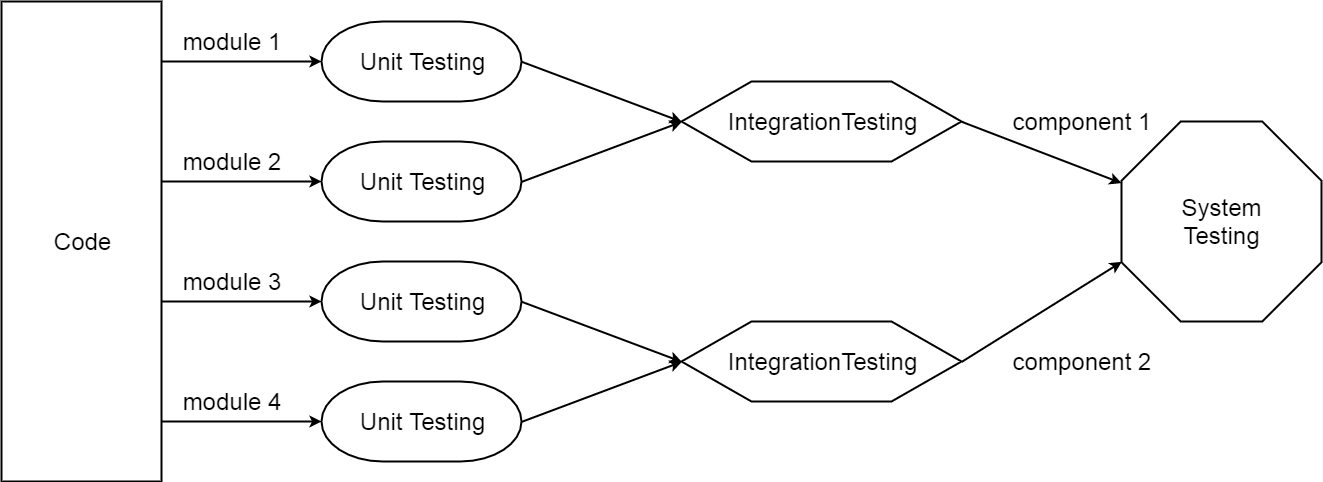
\includegraphics[width=0.8\textwidth]{Testing_process.png}
\end{figure}
\subsubsection{Test Schedule for All Iterations}
\begin{figure}[!htbp]
  \centering 
 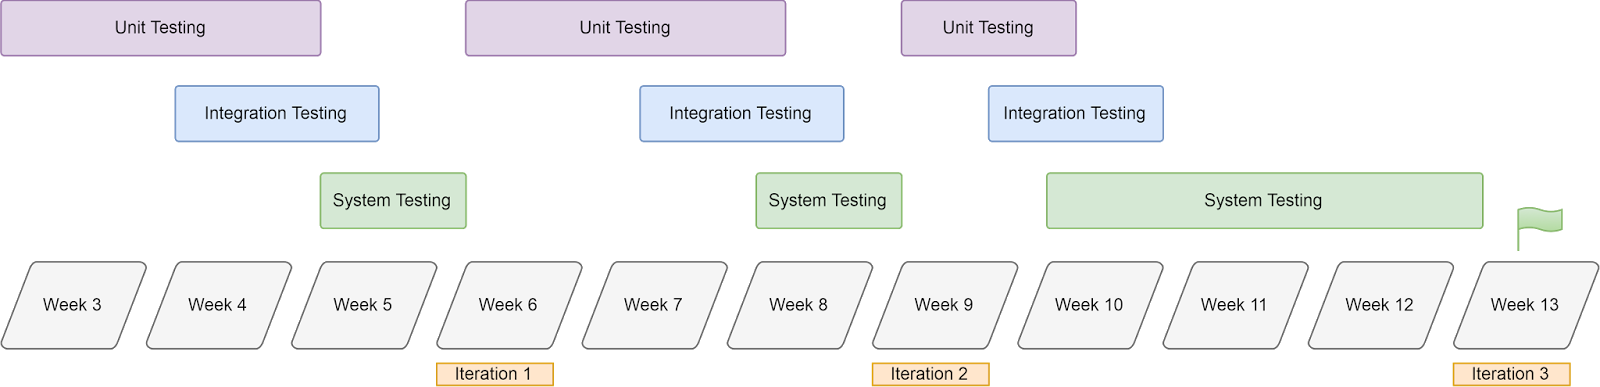
\includegraphics[width=1.0\textwidth]{test_schedule.png}
\end{figure}
For each iteration, unit testing will be conducted during the first half of the iteration, to ensure that the new modules introduced produced the expected result. Algorithms are verified and logical errors will be corrected during this process. Private methods are tested by creating friend classes and accessing them using the these friend classes. Individual developers are responsible for testing their own code. Integrating testing will be conducted to ensure that these modules are able to communicate and interact with other components as expected. For example, tests are written to check whether QueryValidator is able to store data into the QueryTree, and whether the retrieved data from QueryTree are the same as those stored by the QueryValidator. Towards the end of each iteration, system testings are carried out frequently using the AutoTester to check for regression. Two developers are delegated to creating new source programs and generating queries that covers corner cases. At any point during the testing process, bugs that surface will be resolved immediately by the developer of the component.
\subsubsection{Test Objectives}
The following components are the components subjected to testing: 
\begin{figure}[!htbp]
  \centering 
 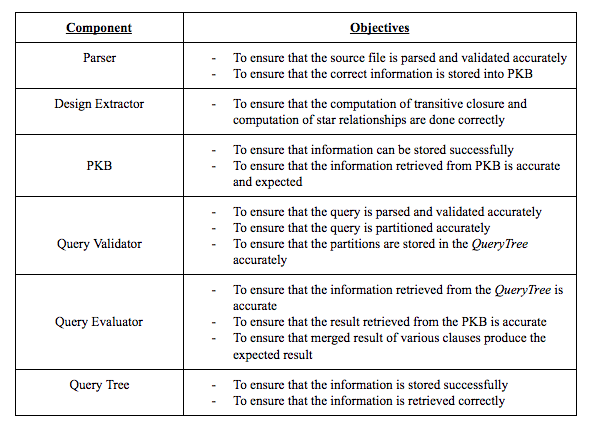
\includegraphics[width=1.1\textwidth]{component_tests.png}
\end{figure}
\subsection{Test Utilities}
\subsubsection{Test Utilities Class}
Test utilities classes provide helper methods to aid the testing process.
\subsubsection{Test Objectives}
The following components are subjected to testing: 
\begin{figure}[!htbp]
  \centering 
 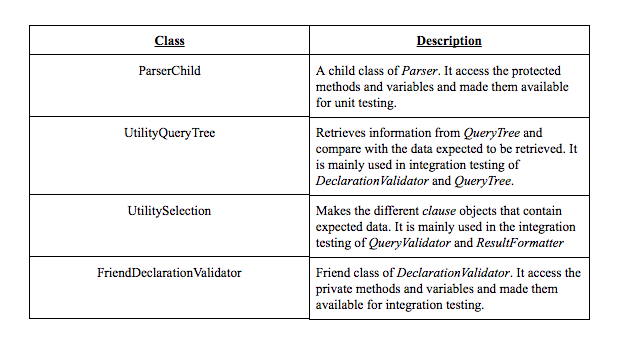
\includegraphics[width=1.1\textwidth]{Test_utilities.png}
\end{figure}
\subsubsection{Script for automating System Testing}
Scripts are created to automate system testing.
\begin{enumerate}
\item Given a SIMPLE source program, a unique excel sheet containing the different queries designed for the source program will be created. 
\begin{figure}[!htbp]
  \centering 
  \caption{Excel sheet containing the queries}
 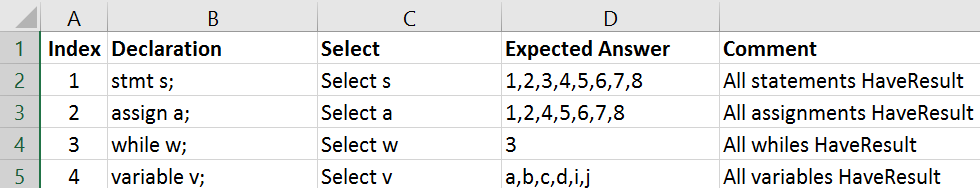
\includegraphics[width=1.1\textwidth]{excel.png}
\end{figure}
\item A python script will convert this excel sheet into a text file so that it can be passed to AutoTester. 
\item A batch file is also written to automatically run the AutoTester.
\begin{figure}[!htbp]
  \centering 
  \caption{Batch file used for automating AutoTester}
 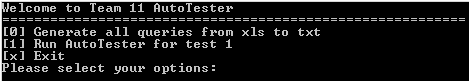
\includegraphics[width=1.1\textwidth]{bat.png}
\end{figure}
\end{enumerate}
\subsection{Unit Tests}
Unit testing involves the testing of individual modules within the component, as well as the component itself, isolated from other components of the system. It is a form of white-box testing, where test cases specifically targets the internal structure of the module.
\subsubsection{PKB Unit Test}
Before the start of the test, pre-defined relationships are injected directly into the PKB table.
\begin{table}[!htbp]
  \centering 
 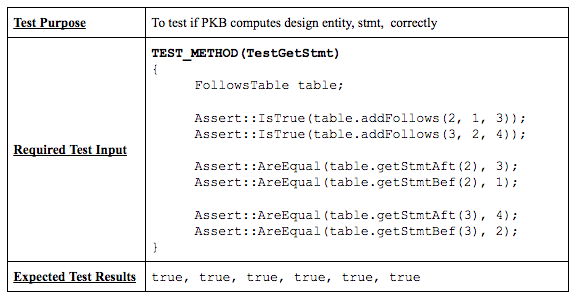
\includegraphics[width=0.7\textwidth]{UnitTest1.png}
\end{table}
\begin{table}[!htbp]
  \centering 
  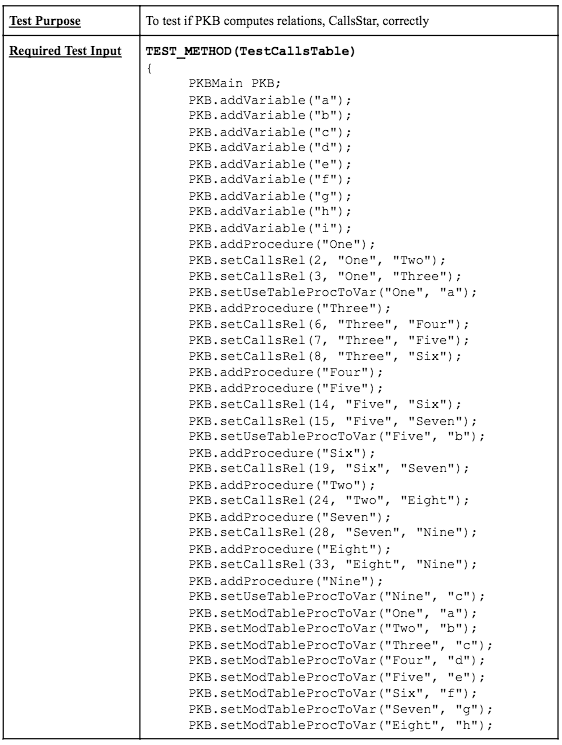
\includegraphics[width=0.8\textwidth]{UnitTest2.png}
\end{table}
\begin{table}[!htbp]
  \centering 
  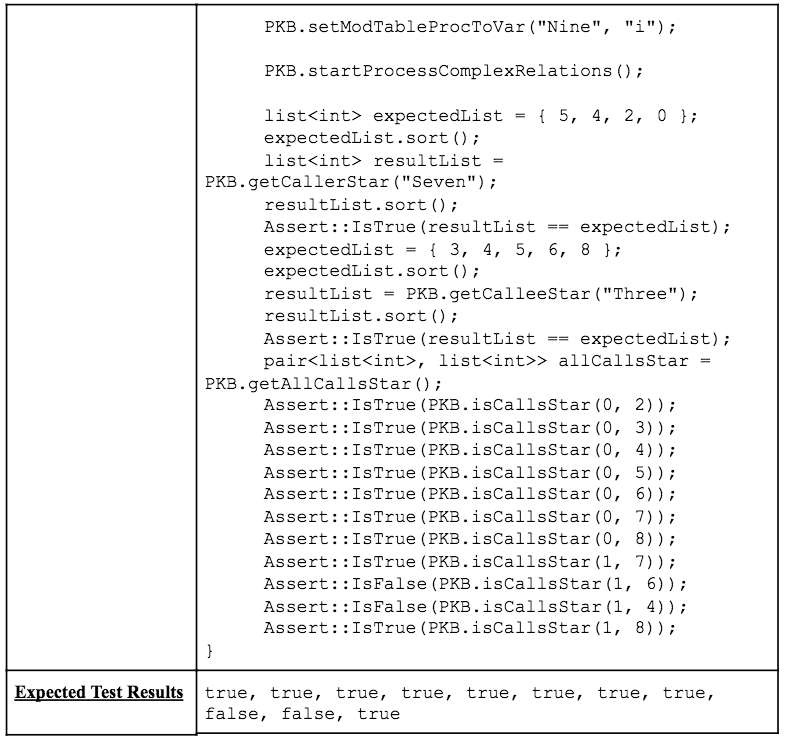
\includegraphics[width=0.8\textwidth]{UnitTest3.png}
\end{table}
\subsubsection{PQL Unit Test}
In PQL Unit testing, the tests are mostly written to test QueryValidator. In particular, the tests targets the accuracy of the regex of each clause. As QueryValidator determines the argument type by enquiring the QueryTree, semantic checks for the types of arguments are done in the integration tests.
\begin{table}[!htbp]
  \centering 
  \caption{Unit Test for PQL}
 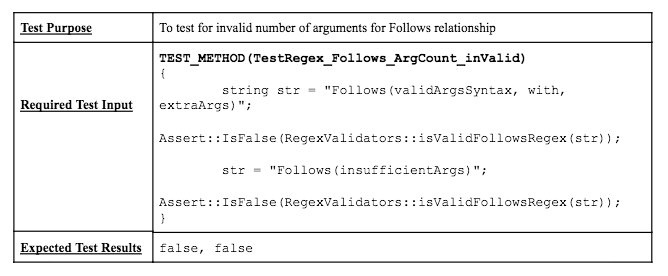
\includegraphics[width=0.7\textwidth]{PQL1.png}
\end{table}
\newline Another example will be testing of ClauseResult used by the QueryEvaluator.
\begin{table}[!htbp]
  \centering 
  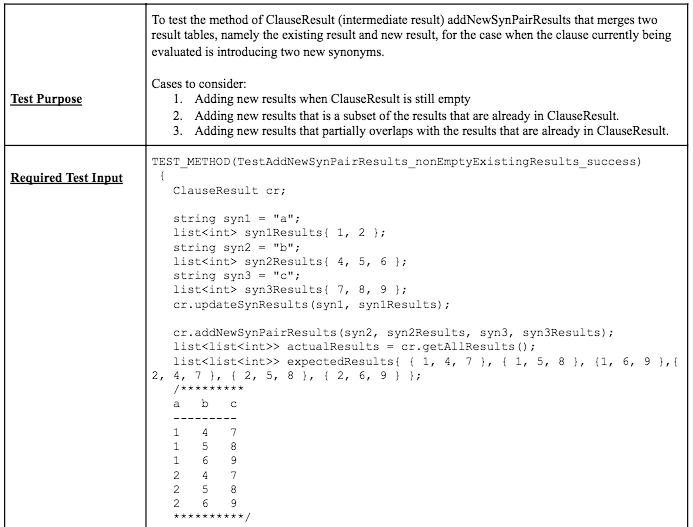
\includegraphics[width=0.8\textwidth]{PQL2.png}
\end{table}
\begin{table}[!htbp]
  \centering 
  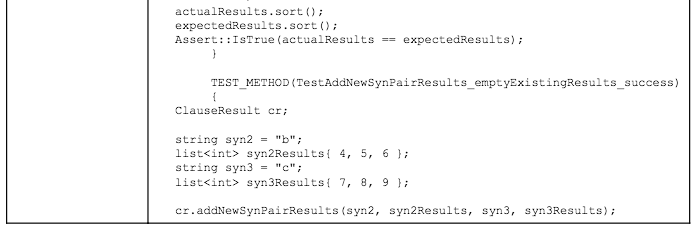
\includegraphics[width=0.8\textwidth]{PQL3.png}
\end{table}
\begin{table}[!htbp]
  \centering 
 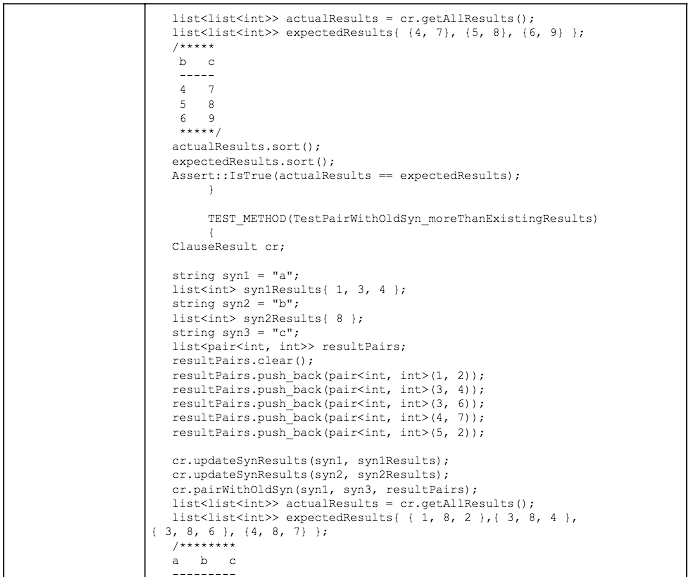
\includegraphics[width=0.7\textwidth]{PQL4.png}
 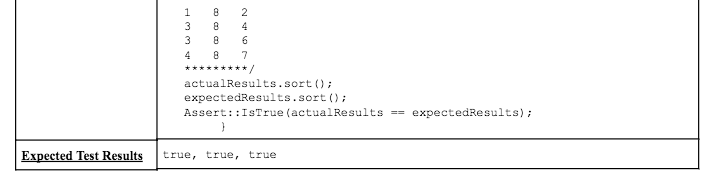
\includegraphics[width=0.737\textwidth]{PQL5.png}
\end{table}
\subsection{Integration Tests}
Integration testing involves the testing of different selected components of the system together. It is assumed that each individual component has been subjected to unit testing.
\begin{figure}[!htbp]
  \centering 
  \caption{Sequence diagram for AutoTester}
 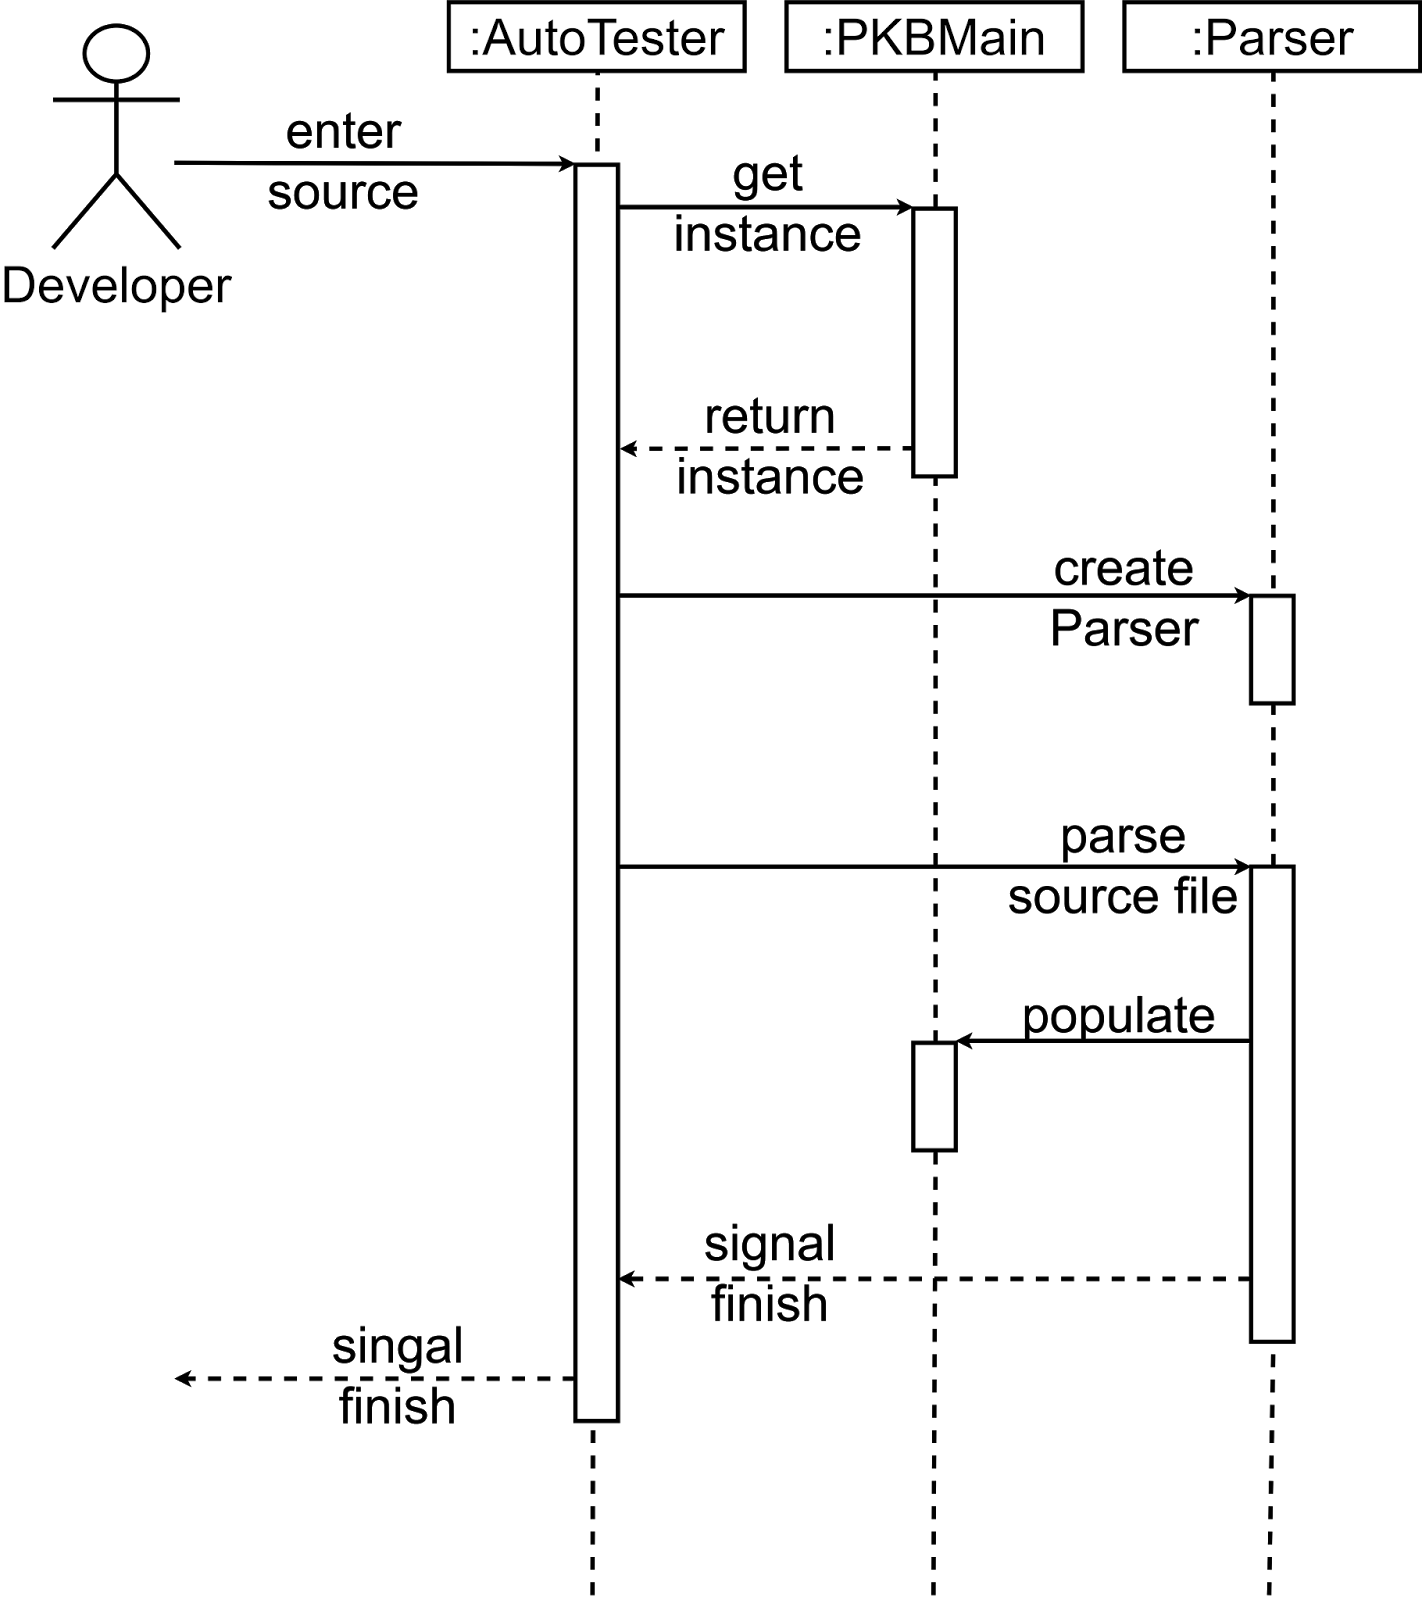
\includegraphics[width=0.7\textwidth]{SDTesting.png}
\end{figure}
\subsubsection{Parser - PKB SubSystem}
Helper methods are created to create dummy SIMPLE source codes and to destroy them at the end of the integration tests.
\begin{figure}[!htbp]
  \centering 
 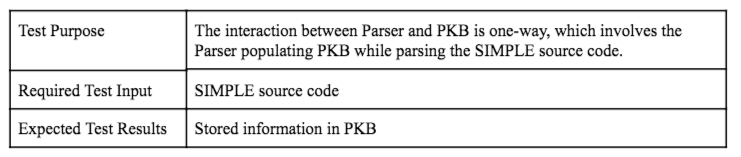
\includegraphics[width=0.7\textwidth]{Testssss.png}
\end{figure}
\newline
After parsing the dummy SIMPLE source codes and populating PKB, actual stored information is extracted using the API of PKB. This extracted data is then compared to expected ones.

\subsubsection{PQL - PKB SubSystem}
\begin{table}[!htbp]
  \centering 
  \caption{Integration Testing}
 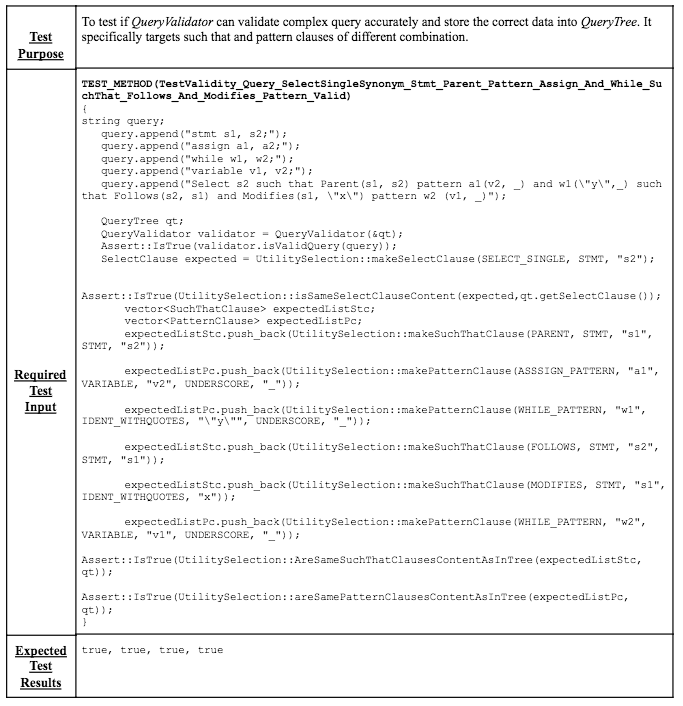
\includegraphics[width=1.0\textwidth]{IntegrationTesting1.png}
\end{table}
 In this example, the components subjected to integration tests are QueryValidator and QueryTree.
\subsection{System Tests}
\begin{table}[!htbp]
  \centering 
  \caption{System Testing}
 \includegraphics[width=0.7\textwidth]{SystemTesting1.png}
\end{table}
System testing involves the testing of all components of the system together. This is carried out with the assistance of the AutoTester. Test cases are designed based on the considerations in Table 9.
As mentioned in the previous section, test cases in system testing are controlled and run via a batch file.
\begin{table}[!htbp]
  \centering 
  \caption{System Tests}
 \includegraphics[width=0.7\textwidth]{SystemTest2.png}
 \includegraphics[width=0.7\textwidth]{SystemTest3.png}
\end{table}
\section{Discussion}
\subsection{Technical Difficulties}
For iteration 2, the technical difficulties were minimal as the team was more used to Visual Studio 2015 and Version Control.
\subsection{Project Management}
We discussed what went wrong in Iteration 1 and how we could improve it with proper project management. We came up with mini-iterations, and scheduled weekly meetings and coded collaboratively in order to ensure optimal working conditions and motivation for each team member to put their best effort in. This way, we were able to input consistent work.
\subsection{Workload and Time Management}
Due to the mid term tests for other modules, our project progress was delayed. However, we managed to catch up with the schedule with proper time management schedule.
One challenge we faced was trying to design an efficient algorithm to compute star relationships such as Follows*, Parent*, Calls*, Next*, using design extractor and CFG. Furthermore, Query Evaluator had to spend a large amount of time coming up with the suggested APIs for the PKB component so that it can deal with multiple complex clauses. However, we were able to discuss the APIs well in time for the deadline.
\section{Future Plan for Iteration 3}
We will continue with the current project management plan we have - develop mini iterations and follow them through.
\subsection{Features}
\textbf{Parser} \newline
For iteration 3, the Parser will be upgraded so that it displays feedback message specific to syntax errors that if detects. \newline

\textbf{Query Validator} \newline
For iteration 3, the QueryValidator will support the validation of relationship Affects and Affects*, as well as the validation of tuple.
\begin{appendices}
\section{Documentation   of   Abstract   APIs} 
Given on the next page.
\end{appendices}
\end{document}